% Introduction to Convex Optimization and Gradient Descent
% Standalone lecture notes modeled on the visible conventions in fft.tex.
% The original course preamble.tex was not supplied, so the small style
% block below defines the lecture, hide, vs, and QU interfaces locally.
%
% Compile twice with: pdflatex convex_optimization.tex
% Instructor version (default): answers and fill-ins are visible.
% Student version: change \studentversionfalse to \studentversiontrue,
% or compile with:
% pdflatex -jobname=convex_optimization_student \
%   '\def\studenthandout{1}% Introduction to Convex Optimization and Gradient Descent
% Standalone lecture notes modeled on the visible conventions in fft.tex.
% The original course preamble.tex was not supplied, so the small style
% block below defines the lecture, hide, vs, and QU interfaces locally.
%
% Compile twice with: pdflatex convex_optimization.tex
% Instructor version (default): answers and fill-ins are visible.
% Student version: change \studentversionfalse to \studentversiontrue,
% or compile with:
% pdflatex -jobname=convex_optimization_student \
%   '\def\studenthandout{1}% Introduction to Convex Optimization and Gradient Descent
% Standalone lecture notes modeled on the visible conventions in fft.tex.
% The original course preamble.tex was not supplied, so the small style
% block below defines the lecture, hide, vs, and QU interfaces locally.
%
% Compile twice with: pdflatex convex_optimization.tex
% Instructor version (default): answers and fill-ins are visible.
% Student version: change \studentversionfalse to \studentversiontrue,
% or compile with:
% pdflatex -jobname=convex_optimization_student \
%   '\def\studenthandout{1}% Introduction to Convex Optimization and Gradient Descent
% Standalone lecture notes modeled on the visible conventions in fft.tex.
% The original course preamble.tex was not supplied, so the small style
% block below defines the lecture, hide, vs, and QU interfaces locally.
%
% Compile twice with: pdflatex convex_optimization.tex
% Instructor version (default): answers and fill-ins are visible.
% Student version: change \studentversionfalse to \studentversiontrue,
% or compile with:
% pdflatex -jobname=convex_optimization_student \
%   '\def\studenthandout{1}\input{convex_optimization.tex}'
%
% Source scope: Part6_main.pdf, Sections 1--2 (main lecture), and
% Section 5.1 (definition of a convex set in the final extension).
% The companion 10-20.pdf supplies the one-dimensional-first progression.
% New numerical examples and questions are practice exercises, not quotations.

\documentclass[11pt,letterpaper]{article}
\usepackage[lmargin=1in,rmargin=1.75in,bmargin=1in,tmargin=1in]{geometry}
\usepackage[T1]{fontenc}
\usepackage{lmodern}
\usepackage{amsmath,amssymb,amsthm}
\usepackage{graphicx}
\usepackage{setspace}
\usepackage{enumitem}
\usepackage{algorithm}
\usepackage{algpseudocode}
\usepackage{float}
\usepackage{tikz}
\usepackage{environ}
\usepackage{fancyhdr}
\usepackage{microtype}
\usepackage[hidelinks]{hyperref}
\usetikzlibrary{arrows.meta}

% ---------------- Editable course information ----------------
\newcommand{\CourseName}{CSCE 411: Design and Analysis of Algorithms}
\newcommand{\LectureDate}{} % Fill in the actual lecture date here.
\newcommand{\LectureNumber}{} % Optional, e.g., 15: (include the colon).

% ---------------- Standalone course-style definitions ----------------
\newif\ifstudentversion
\studentversionfalse
\ifdefined\studenthandout\studentversiontrue\fi
\newcommand{\vs}[1]{\vspace{#1}}
\newcommand{\hide}[1]{%
  \ifstudentversion
    \ifmmode\phantom{#1}\else\underline{\phantom{#1}}\fi
  \else #1\fi}
\newcommand{\lecture}[2]{%
  \noindent\textbf{\CourseName}\hfill #2\par
  \vspace{5pt}\hrule\vspace{10pt}
  {\centering\Large\bfseries #1\par}
  \vspace{10pt}\hrule\vspace{9pt}}
\theoremstyle{definition}
\newtheorem{definition}{Definition}
\newtheorem{example}{Example}
\theoremstyle{plain}
\newtheorem{lemma}{Lemma}
\newtheorem{theorem}{Theorem}
\newtheorem{fact}{Fact}
\newcounter{question}
\newenvironment{Qu}{%
  \par\medskip\refstepcounter{question}
  \noindent\textbf{Question \thequestion.}\ }{\par\medskip}
\newcommand{\QU}{\begin{Qu}}
\newcommand{\aitem}{\item[\textbf{(A)}]}
\newcommand{\bitem}{\item[\textbf{(B)}]}
\newcommand{\citem}{\item[\textbf{(C)}]}
\newcommand{\ditem}{\item[\textbf{(D)}]}
\newcommand{\eitem}{\item[\textbf{(E)}]}
\newsavebox{\answerbox}
% Answers occupy the same space in both versions; in the student version
% this space is left blank for the in-class calculation or discussion.
\NewEnviron{answer}{%
  \par\begingroup
  \setbox\answerbox=\vbox{\hsize=\linewidth\parindent=0pt\BODY\par}%
  \noindent\ifstudentversion\phantom{\usebox{\answerbox}}%
  \else\usebox{\answerbox}\fi\par\endgroup}
\newenvironment{problemframe}{%
  \par\smallskip\noindent
  \begin{lrbox}{\answerbox}
  \begin{minipage}{\dimexpr\linewidth-2\fboxsep-2\fboxrule\relax}}%
  {\end{minipage}\end{lrbox}\fbox{\usebox{\answerbox}}\par\smallskip}
\newcommand{\R}{\mathbb R}
\newcommand{\X}{\mathcal X}
\newcommand{\eps}{\varepsilon}
\newcommand{\xstar}{x^\star}
\DeclareMathOperator*{\argmin}{arg\,min}
\setlength{\parindent}{0pt}
\setlength{\parskip}{5pt}
\setlength{\headheight}{14pt}
\setlist[itemize]{topsep=3pt,itemsep=2pt,parsep=0pt}
\setlist[enumerate]{topsep=3pt,itemsep=2pt,parsep=0pt,leftmargin=2.1em}
\pagestyle{fancy}
\fancyhf{}
\fancyhead[L]{\small Convex Optimization and Gradient Descent}
\fancyhead[R]{\small CSCE 411}
\fancyfoot[C]{\thepage}
\renewcommand{\headrulewidth}{0.3pt}
\renewcommand{\footrulewidth}{0pt}
\raggedbottom
\hypersetup{pdftitle={Introduction to Convex Optimization and Gradient Descent},
  pdfauthor={CSCE 411 Lecture Notes},pdfsubject={Design and Analysis of Algorithms}}

\begin{document}
\onehalfspacing
\thispagestyle{plain}

% ======================== PAGE 1 ========================
\lecture{\LectureNumber\ Introduction to Convex Optimization\\and Gradient Descent}{\LectureDate}

\paragraph{Reading.}
Kevin Tian, \emph{Part VI: Continuous Algorithms}, Sections 1--2;
and the accompanying October 20 lecture notes. The last section briefly
introduces the higher-dimensional viewpoint from Section 5.1.

\section{Motivation: From Discrete to Continuous Optimization}

Many problems we have studied ask us to choose the best object from a set of
possible objects. We can write this common form as
\[
  \min_{x\in\X} f(x)
  \qquad\text{or}\qquad
  \max_{x\in\X} f(x).
\]
The variable $x$ is the \hide{\textbf{decision variable}}, the set $\X$ is the
\hide{\textbf{feasible set}}, and $f$ is the \hide{\textbf{objective function}}.

\begin{center}
\renewcommand{\arraystretch}{1.25}
\begin{tabular}{lll}
\textbf{Problem} & \textbf{Feasible objects} & \textbf{Objective}\\\hline
Interval scheduling & Nonoverlapping subsets & Maximize subset size\\
Minimum spanning tree & Spanning trees & Minimize total weight\\
Shortest path & $s$--$t$ paths & Minimize total weight
\end{tabular}
\end{center}

In these examples, the choices are discrete. Today, the decision variable
can instead be a real number or a vector of real numbers: $x\in\X\subseteq\R^d$.
There may be infinitely many feasible choices!

\begin{example}\textbf{Approximate Continuous Minimization}
\begin{problemframe}
\textbf{Input:} A function $f:\X\to\R$, a nonempty feasible set
$\X\subseteq\R^d$, and an accuracy parameter $\eps>0$.

\textbf{Output:} A point $\widehat x\in\X$ satisfying
\[
  f(\widehat x)\leq \hide{f(\xstar)+\eps},
  \qquad \xstar\in\argmin_{x\in\X} f(x).
\]
Here we assume that a minimizer $\xstar$ exists.
\end{problemframe}
\end{example}

Our accuracy target concerns the \emph{objective value}, not necessarily the
location of the output. An additive error of $\eps$ need not imply
$|\widehat x-\xstar|\leq\eps$.

% ======================== PAGE 2 ========================
\newpage
\subsection{A Familiar Example: Maximum Flow}

A maximum-flow problem already has a continuous formulation. Let
$G=(V,E)$ be a directed graph, with source $s$, sink $t$, and capacities
$c_e\geq0$. For this formulation, assume no edges enter $s$ or leave $t$.
Let $x_e$ denote the flow on edge $e$, so the decision variable is
$x\in\R^{|E|}$.

We want to maximize
\[
  f(x)=\sum_{e=(s,v)\in E}x_e
\]
subject to the constraints
\begin{align*}
  0\leq x_e&\leq c_e &&\text{for every }e\in E,\\
  \sum_{e=(u,v)\in E}x_e&=
  \sum_{e=(v,w)\in E}x_e &&\text{for every }v\in V\setminus\{s,t\}.
\end{align*}
The first constraints enforce \hide{capacity bounds}; the second enforce
\hide{flow conservation}. The feasible set $\X$ contains every flow satisfying
these constraints.

\QU Suppose there is a nonzero feasible flow $x$. Why are there infinitely
many feasible flows, even though the graph is finite?
\end{Qu}
\begin{answer}
For every $\lambda\in[0,1]$, the scaled flow $\lambda x$ is feasible:
capacity inequalities and conservation are preserved. Because $x\neq0$,
different values of $\lambda$ give different flows.
\end{answer}
\vs{0.25in}

\subsection{Another Motivation: Fitting a Model to Data}

Suppose $x\in\R^d$ records the parameters of a prediction rule. We can use a
\textbf{loss function} $f(x)$ to measure its errors on a collection of
training examples, and choose the parameters by minimizing $f(x)$.

There are infinitely many parameter choices, so enumerating all models is
not an option. Instead, we will repeatedly improve a current guess using
local information about the objective.

\textbf{Important distinction.} The loss of a complicated model need not be
convex. Our analysis will separate what smoothness alone guarantees from
what additionally requires convexity.

% ======================== PAGE 3 ========================
\newpage
\section{What Information Can an Algorithm Use?}

In the \hide{\textbf{oracle model}}, we ask for information about $f$ at
points of our choice. A \textbf{value query} returns $f(x)$; a
\textbf{derivative query} returns $f'(x)$ in one dimension.
We count queries separately from the cost of computing them.
For the gradient-descent theorems, we assume exact derivative queries and
exact real arithmetic.

Derivative queries are natural because a derivative describes how the
function changes nearby. Value queries can also \emph{approximate} a
derivative through
\[
  f'(x)\approx\frac{f(x+\delta)-f(x)}{\delta},
  \qquad \delta>0.
\]
We will make the approximation error precise after defining smoothness.

\subsection{Without Structure, Queries May Tell Us Nothing}

For an unknown point $z\in[0,1]$, consider
\[
  f_z(x)=
  \begin{cases}
    0,&x=z,\\
    1,&x\neq z.
  \end{cases}
\]
Even finding $\widehat x$ with $f_z(\widehat x)\leq\min f_z+0.99$ requires
finding \hide{the exact point $z$}.

\textbf{Why finitely many queries cannot guarantee success.}
Consider a deterministic algorithm and answer every query with $1$.
After its finite query sequence and output $\widehat x$, choose $z$ outside
all queried points and outside $\{\widehat x\}$. Every answer is consistent
with $f_z$, but the output has value $1$ while the minimum is $0$.

\textbf{Takeaway:} A bounded domain and bounded function values are not
enough. We need assumptions under which queries provide useful information.

\paragraph{A contrasting example: unimodality.}
If $f$ is strictly decreasing up to a minimizer $c$ and strictly increasing
afterward, compare its values at
\[
  u=\ell+\frac{r-\ell}{3},\qquad
  v=\ell+\frac{2(r-\ell)}{3}
\]
in a known interval $[\ell,r]$ containing $c$. If $f(u)<f(v)$, discard
$(v,r]$; if $f(u)>f(v)$, discard $[\ell,u)$; if they are equal, retain $[u,v]$.
This is \hide{\textbf{ternary search}}: local queries now reveal which
part of the interval can contain the minimizer.

% ======================== PAGE 4 ========================
\newpage
\section{Convexity: Structure That Helps Optimization}

We first work in \textbf{one dimension}. Unless otherwise specified,
$f:\R\to\R$, and we minimize over all of $\R$.

\begin{definition}
A function $f:\R\to\R$ is \hide{\textbf{convex}} if, for every $x,y\in\R$
and every $\lambda\in[0,1]$,
\[
  \boxed{f((1-\lambda)x+\lambda y)
  \leq (1-\lambda)f(x)+\lambda f(y).}
\]
\end{definition}

The point $(1-\lambda)x+\lambda y$ is a weighted average of $x$ and $y$.
The right-hand side is the height of the line segment joining
$(x,f(x))$ and $(y,f(y))$. A convex function lies \hide{at or below}
every such segment.

\begin{center}
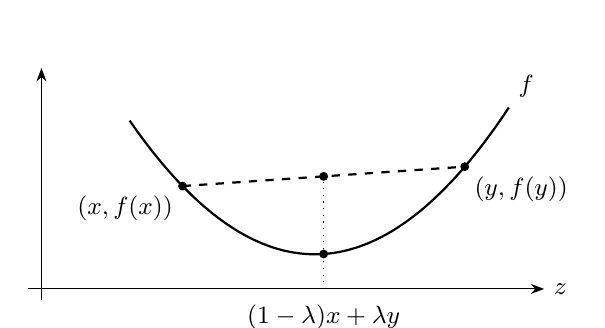
\begin{tikzpicture}[x=1.12cm,y=1.1cm,>=Stealth,font=\small]
  \draw[->] (-1.25,0)--(4.6,0) node[right] {$z$};
  \draw[->] (-1.1,-0.13)--(-1.1,2.55);
  \draw[thick,domain=-0.1:4.2,samples=90]
    plot (\x,{0.35*(\x-2)^2+0.4});
  \draw[thick,dashed] (0.5,1.1875)--(3.7,1.4115);
  \fill (0.5,1.1875) circle(1.6pt) node[below left] {$(x,f(x))$};
  \fill (3.7,1.4115) circle(1.6pt) node[below right] {$(y,f(y))$};
  \draw[dotted] (2.1,0)--(2.1,1.2995);
  \fill (2.1,0.4035) circle(1.6pt);
  \fill (2.1,1.2995) circle(1.6pt);
  \node[below,align=center] at (2.1,-0.07) {$(1-\lambda)x+\lambda y$};
  \node[above right] at (4.2,2.094) {$f$};
\end{tikzpicture}
\end{center}

\QU Which of the following functions are convex on $\R$?
\[
  f_1(x)=x^2,\quad f_2(x)=|x|,\quad
  f_3(x)=3x+1,\quad f_4(x)=-x^2.
\]
\begin{enumerate}
  \aitem Only $f_1$.
  \bitem Only $f_1$ and $f_2$.
  \citem $f_1$, $f_2$, and $f_3$.
  \ditem All four functions.
\end{enumerate}
\end{Qu}
% Answer: C.
\begin{answer}
\textbf{Answer: C.} Convex functions need not be differentiable: $|x|$ has a
corner at $0$. Linear functions satisfy the convexity inequality with
equality. For $-x^2$, take $x=-1$, $y=1$, and $\lambda=1/2$:
the proposed inequality would be $0\leq-1$.
\end{answer}

% ======================== PAGE 5 ========================
\newpage
\subsection{A Second View: Convex Functions Lie Above Their Tangents}

If $f$ is differentiable, its linear, or \textbf{Euler}, approximation at
$x$ is
\[
  f(x)+f'(x)(y-x).
\]
For a general function, this is only a local approximation. For a convex
function, it gives a \hide{global lower bound}.

\begin{lemma}[First-order inequality]\label{lem:convexity}
If $f:\R\to\R$ is differentiable and convex, then, for all $x,y\in\R$,
\[
  \boxed{f(y)\geq f(x)+f'(x)(y-x).}
\]
\end{lemma}

\begin{proof}
For $0<\lambda\leq1$, convexity gives
\[
  f(x+\lambda(y-x))\leq(1-\lambda)f(x)+\lambda f(y).
\]
Rearrange, dividing by the positive number $\lambda$:
\[
  f(y)\geq f(x)+\frac{f(x+\lambda(y-x))-f(x)}{\lambda}.
\]
Let $\lambda\to0^+$. The quotient tends to
\hide{$f'(x)(y-x)$}, which proves the inequality.
\end{proof}

\vs{0.2in}
\textbf{Two compatible pictures of convexity:}
\[
  \text{below every \hide{chord}}
  \qquad\text{and}\qquad
  \text{above every \hide{tangent}}.
\]

\QU Suppose $f$ is differentiable and convex, and $f'(x)=0$.
What can we conclude?
\begin{enumerate}
  \aitem $x$ is necessarily the unique minimizer.
  \bitem $x$ is a global minimizer, but need not be unique.
  \citem $x$ could be a strict local maximum.
  \ditem Nothing about optimality.
\end{enumerate}
\end{Qu}
% Answer: B.
\begin{answer}
\textbf{Answer: B.} For every $y$, the first-order inequality yields
$f(y)\geq f(x)+0\cdot(y-x)=f(x)$. A constant function shows that the
minimizer need not be unique.
\end{answer}

% ======================== PAGE 6 ========================
\newpage
\subsection{Why Local Information Is Useful}

\begin{lemma}[Local minima are global minima]
For a convex function, every local minimum is a global minimum.
\end{lemma}
\begin{proof}
Suppose $x$ is a local minimum but $f(y)<f(x)$ for some $y$.
For sufficiently small $\lambda>0$, the point
$z=(1-\lambda)x+\lambda y$ lies in the neighborhood where $x$ is a minimum.
But
\[
  f(z)\leq(1-\lambda)f(x)+\lambda f(y)<f(x),
\]
which is a contradiction. This argument does not require differentiability.
\end{proof}

\paragraph{The derivative points toward improvement.}
Let $\xstar$ be a minimizer. If $f'(x)>0$, then, for every $y>x$,
\[
  f(y)\geq f(x)+f'(x)(y-x)>f(x).
\]
Thus no minimizer lies to the \hide{right} of $x$. Similarly, if
$f'(x)<0$, no minimizer lies to the \hide{left} of $x$.
Given an interval containing a minimizer, these tests permit binary search.
If $f'(x)=0$, we have already found a global minimizer.

\begin{fact}[Calculus test]
For twice-differentiable $f:\R\to\R$, convexity is equivalent to
$f''(x)\geq0$ for all $x$. Equivalently, $f'$ is nondecreasing.
\end{fact}

\section{Gradient Descent: Move Instead of Discard}

A one-dimensional interval has a natural left and right. In high dimensions,
there is no direct analogue of this interval-based binary search.
An alternative is to move our current point using its derivative:
\[
  \boxed{x_{t+1}=x_t-\eta f'(x_t).}
\]
This is \hide{\textbf{gradient descent}}. The parameter $\eta>0$ is the
\hide{\textbf{step size}}.

\textbf{The design question:} How should we choose $\eta$? Too small may
mean very slow progress; too large may overshoot the minimizer and even
increase the objective. Moving in a descent direction is not, by itself,
a guarantee that an arbitrary-length step decreases $f$.

% ======================== PAGE 7 ========================
\newpage
\section{Smoothness: How Far Can We Safely Move?}

We need a condition that prevents the derivative from changing too quickly.
First, recall a related condition on function values.

\begin{definition}
Let $G\geq0$ and $L>0$. A function $f:\R\to\R$ is
\textbf{$G$-Lipschitz} if, for all $x,y\in\R$,
\[
  |f(x)-f(y)|\leq G|x-y|.
\]
A differentiable function $f:\R\to\R$ is \textbf{$L$-smooth} if, for all
$x,y\in\R$,
\[
  \boxed{|f'(x)-f'(y)|\leq L|x-y|.}
\]
\end{definition}

Lipschitzness of $f$ controls its \hide{values}; smoothness controls its
\hide{derivative}. We use $G$ and $L$ to distinguish these two bounds.

\textbf{Useful calculus tests.} On $\R$, for differentiable $f$,
$|f'|\leq G$ everywhere is equivalent to $G$-Lipschitzness.
For twice-differentiable $f$, $|f''|\leq L$ everywhere is equivalent to
$L$-smoothness.

\QU Classify each function on \emph{all of $\R$}.
\begin{center}
\renewcommand{\arraystretch}{1.35}
\begin{tabular}{lccc}
 & \textbf{Convex?} & \textbf{Lipschitz?} & \textbf{Smooth?}\\\hline
$x^2$ & \hide{Yes} & \hide{No} & \hide{Yes, $L=2$}\\
$|x|$ & \hide{Yes} & \hide{Yes, $G=1$} & \hide{No}\\
$\cos x$ & \hide{No} & \hide{Yes, $G=1$} & \hide{Yes, $L=1$}
\end{tabular}
\end{center}
\end{Qu}

\paragraph{What about simulating derivative queries?}
For $L$-smooth $f$ and $\delta>0$, the fundamental theorem of calculus gives
\begin{align*}
 \left|\frac{f(x+\delta)-f(x)}{\delta}-f'(x)\right|
 &\leq\frac{1}{\delta}\int_0^\delta|f'(x+s)-f'(x)|\,ds\\
 &\leq\frac{1}{\delta}\int_0^\delta Ls\,ds
 =\frac{L\delta}{2}.
\end{align*}
This is an \emph{approximation}, not an exact simulation. Our theorems use
exact derivative queries; finite-difference and floating-point errors are
not included in those guarantees.

% ======================== PAGE 8 ========================
\newpage
\section{Gradient Descent, Take 1: Quadratics}

The simplest smooth convex functions are quadratics. Let
\[
  q(x)=ax^2+bx+c,\qquad a>0.
\]
We can analyze gradient descent exactly in this case.

\paragraph{Where is the minimizer?}
Complete the square:
\begin{align*}
  q(x)
  &=a\left(x+\frac{b}{2a}\right)^2+c-\frac{b^2}{4a},\\[4pt]
  \xstar&=\hide{-\frac{b}{2a}}.
\end{align*}
The additive constant does not affect the location of the minimizer.
The error in the objective value is
\[
  q(x)-q(\xstar)=\hide{a(x-\xstar)^2}.
\]

\paragraph{What does the derivative tell us?}
\[
  q'(x)=2ax+b=\hide{2a(x-\xstar)}.
\]
Thus the derivative is exactly proportional to the signed distance from
the current point to the minimizer. Moreover,
\[
  |q'(x)-q'(y)|=2a|x-y|,
\]
so the tight smoothness constant is \hide{$L=2a$}.

\begin{example}\textbf{Complete the Square}
Let $q(x)=x^2-6x+10$. Find the minimizer, the minimum value, the derivative,
and a tight smoothness constant.
\end{example}
\begin{answer}
\begin{align*}
  q(x)&=(x-3)^2+1,&\xstar&=3,\\
  q(\xstar)&=1,&q'(x)&=2x-6,\qquad L=2.
\end{align*}
\end{answer}
\vs{0.4in}

\textbf{Next question:} Can we choose a step size that lands directly at
$\xstar$?

% ======================== PAGE 9 ========================
\newpage
\subsection{Choosing and Testing the Step Size}

For a quadratic with tight smoothness constant $L=2a$, a gradient step is
\[
  x_{t+1}=x_t-\eta L(x_t-\xstar).
\]
Subtracting $\xstar$ from both sides gives the exact recurrence
\[
  \boxed{x_{t+1}-\xstar=(1-\eta L)(x_t-\xstar).}
\]
With $\eta=\hide{1/L}$, the multiplier is zero: we reach the minimizer in
\hide{one step}. A larger valid upper bound on smoothness gives a smaller,
still safe step, but need not give one-step convergence.

\begin{example}\textbf{Trace the Iterates}
Use $q(x)=x^2-6x+10$, $x_0=0$, and $L=2$. Compute $x_1$ and $x_2$ for each
choice of $\eta$.
\begin{center}
\renewcommand{\arraystretch}{1.6}
\begin{tabular}{c|cc|l}
$\eta$ & $x_1$ & $x_2$ & \textbf{Behavior}\\\hline
$1/4$ & \hide{$3/2$} & \hide{$9/4$} & \hide{Approaches from one side}\\
$1/2$ & \hide{$3$} & \hide{$3$} & \hide{Reaches the minimizer}\\
$3/4$ & \hide{$9/2$} & \hide{$9/4$} & \hide{Alternates, but gets closer}\\
$1$ & \hide{$6$} & \hide{$0$} & \hide{Oscillates without progress}
\end{tabular}
\end{center}
\end{example}

\QU Does overshooting always imply that gradient descent diverges?
Use the recurrence to determine exactly when the distance decreases
for this quadratic.
\end{Qu}
\begin{answer}
No. The distance decreases at every nonoptimal iterate precisely when
\[
  |1-\eta L|<1\quad\Longleftrightarrow\quad 0<\eta<\frac{2}{L}.
\]
For $1/L<\eta<2/L$, the iterates cross the minimizer but get closer.
At $\eta=2/L$, a nonoptimal starting point oscillates. For $\eta>2/L$, its
distance grows. Thus $1/L$ is a convenient safe choice, not the only
convergent choice for a quadratic.
\end{answer}
\vs{0.15in}

\textbf{Progress with $\eta=1/L$:}
\[
  q(x)-q\left(x-\frac{q'(x)}{L}\right)
  =a(x-\xstar)^2=\hide{\frac{(q'(x))^2}{2L}}.
\]

% ======================== PAGE 10 ========================
\newpage
\section{Gradient Descent, Take 2: Smooth Functions}

A general smooth function is not a quadratic. The useful replacement is
that it has a \textbf{quadratic upper bound} centered at every point.

\begin{lemma}[Quadratic upper bound]\label{lem:smooth}
If $f:\R\to\R$ is $L$-smooth, then, for every $x,y\in\R$,
\[
  \boxed{f(y)\leq f(x)+f'(x)(y-x)+\frac L2(y-x)^2.}
\]
Convexity is \emph{not} required.
\end{lemma}

\textbf{Intuition.} A first-order approximation uses the tangent line.
Smoothness controls how far the derivative can move away from its initial
value, so the error accumulated along a step is at most quadratic in the
step length.

\begin{proof}
Write $h=y-x$. Parameterizing the segment from $x$ to $y$ by $x+sh$, where
$0\leq s\leq1$, gives
\begin{align*}
 f(y)-f(x)-f'(x)h
   &=\int_0^1\bigl(f'(x+sh)-f'(x)\bigr)h\,ds\\
   &\leq\int_0^1|f'(x+sh)-f'(x)|\,|h|\,ds\\
   &\leq\int_0^1 Ls|h|^2\,ds\\
   &=\hide{\frac L2 h^2}.
\end{align*}
The absolute values make the argument valid whether $y\geq x$ or $y<x$.
Substitute $h=y-x$ and rearrange.
\end{proof}

\vs{0.25in}
For a function that is \emph{both convex and $L$-smooth}, we now have
\begin{align*}
  f(x)+f'(x)(y-x)
  &\leq f(y)\\
  &\leq f(x)+f'(x)(y-x)+\frac L2(y-x)^2.
\end{align*}
Convexity supplies the \hide{linear lower bound}.\\
Smoothness supplies the \hide{quadratic upper bound}.\\
These two inequalities play different roles in the analysis.

% ======================== PAGE 11 ========================
\newpage
\subsection{Minimize the Upper Bound, Not the Unknown Function}

At the current point $x$, define the quadratic model
\[
  Q_x(y)=f(x)+f'(x)(y-x)+\frac L2(y-x)^2.
\]
We know $Q_x(x)=f(x)$ and $f(y)\leq Q_x(y)$ for all $y$.

\begin{center}
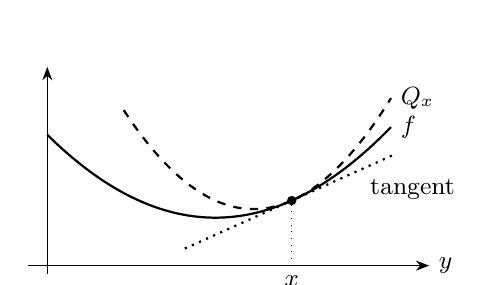
\begin{tikzpicture}[x=0.97cm,y=0.87cm,>=Stealth,font=\small]
  \draw[->] (-2.45,0)--(2.8,0) node[right] {$y$};
  \draw[->] (-2.2,-0.12)--(-2.2,2.9);
  % f(y)=0.25*y^2+0.7, anchor x=1, and a valid L=1 upper model.
  \draw[thick,domain=-2.2:2.3,samples=90]
    plot (\x,{0.25*(\x)^2+0.7});
  \draw[dashed,thick,domain=-1.2:2.3,samples=90]
    plot (\x,{0.95+0.5*(\x-1)+0.5*(\x-1)^2});
  \draw[dotted,thick] (-0.4,0.25)--(2.35,1.625);
  \fill (1,0.95) circle(1.7pt);
  \draw[dotted] (1,0)--(1,0.95);
  \node[below] at (1,0) {$x$};
  \node[right] at (2.3,2.445) {$Q_x$};
  \node[right] at (2.3,2.0225) {$f$};
  \node[below right] at (1.9,1.4) {tangent};
\end{tikzpicture}
\end{center}

Differentiate the quadratic model with respect to $y$:
\[
  Q_x'(y)=f'(x)+L(y-x).
\]
Setting this equal to zero gives its minimizer
\[
  y=\hide{x-\frac{f'(x)}{L}}.
\]
Thus gradient descent with $\eta=1/L$ minimizes a valid quadratic upper
bound at every iteration.

\begin{lemma}[One-step progress]\label{lem:descent}
For any $L$-smooth $f$, the point $x^+=x-f'(x)/L$ satisfies
\[
  \boxed{f(x^+)\leq f(x)-\frac{(f'(x))^2}{2L}.}
\]
\end{lemma}
\begin{proof}
Substitute $y=x-f'(x)/L$ into Lemma~\ref{lem:smooth}:
\[
 f(x^+)\leq f(x)-\frac{(f'(x))^2}{L}
              +\frac{L}{2}\frac{(f'(x))^2}{L^2}
          =f(x)-\frac{(f'(x))^2}{2L}.
\]
\end{proof}

% ======================== PAGE 12 ========================
\newpage
\section{The Algorithm and Its Two Possible Guarantees}

\begin{algorithm}[H]
\caption{Gradient-Descent$(f,x_0,L,T)$}\label{alg:gd}
\begin{algorithmic}[1]
  \Require Derivative access to an $L$-smooth function $f:\R\to\R$;
     $L>0$; initial point $x_0$; integer $T\geq1$
  \State $g_{\mathrm{best}}\gets+\infty$
  \For{$t=0,1,\ldots,T-1$}
    \State $g_t\gets f'(x_t)$
    \If{$|g_t|<g_{\mathrm{best}}$}
      \State $\widehat x\gets x_t$; $g_{\mathrm{best}}\gets |g_t|$
    \EndIf
    \State $x_{t+1}\gets x_t-g_t/L$
  \EndFor
  \State \Return $x_T$ and $\widehat x$
\end{algorithmic}
\end{algorithm}

\textbf{Which output?} We use $\widehat x$ for a small-derivative guarantee,
and $x_T$ for the convex objective-value guarantee. There is no need to
store all previous iterates: retaining the current point and the best
observed derivative magnitude is enough.

\textbf{Runtime.} The algorithm makes \hide{$T$} derivative queries.
If one derivative costs $C_{\mathrm{grad}}$ time, the total time is
\hide{$O(T(C_{\mathrm{grad}}+1))$} in the real-arithmetic model.

\begin{definition}
A point $x$ is an \textbf{$\eps$-critical point} if $|f'(x)|\leq\eps$.
A point $x$ is an \textbf{$\eps$-approximate minimizer} if
$f(x)-f(\xstar)\leq\eps$.
\end{definition}

These are \textbf{different guarantees}. Smoothness alone will let us find
an approximate critical point. Convexity and a distance bound will connect
criticality to global optimality.

\QU Let $f(x)=\cos x$. Gradient descent starts at $x_0=0$.
What happens, and is the output a local minimum?
\end{Qu}
\begin{answer}
Since $f'(0)=-\sin0=0$, every iterate remains at $0$.
But $f(0)=1$ is a global maximum, while $f(\pi)=-1$.
The function is $1$-smooth. Thus even an exactly critical point need not
be a local minimum of a smooth, nonconvex function.
\end{answer}
\vs{0.2in}

\textbf{Scope reminder.} We are minimizing over $\R$. At the boundary of a
constrained feasible set, an optimum need not have derivative zero.

% ======================== PAGE 13 ========================
\newpage
\section{Analysis I: Finding an Approximate Critical Point}

\begin{theorem}[Smooth, possibly nonconvex objective]\label{thm:critical}
Let $f:\R\to\R$ be $L$-smooth, with a minimizer $\xstar$, and suppose $\Delta\geq0$ satisfies
\[
  f(x_0)-f(\xstar)\leq\Delta.
\]
After $T\geq1$ iterations of Algorithm~\ref{alg:gd},
\[
  \boxed{\min_{0\leq t<T}|f'(x_t)|
          \leq\sqrt{\frac{2L\Delta}{T}}.}
\]
In particular, $T\geq 2L\Delta/\eps^2$ suffices for the returned
$\widehat x$ to be an $\eps$-critical point.
\end{theorem}

\textbf{Proof idea.} A large derivative forces a substantial decrease in
$f$. But the total decrease cannot exceed the initial gap $\Delta$.

\begin{proof}
By Lemma~\ref{lem:descent}, for every $0\leq t<T$,
\[
  \frac{(f'(x_t))^2}{2L}\leq f(x_t)-f(x_{t+1}).
\]
Sum over the $T$ iterations. The right-hand side telescopes:
\begin{align*}
  \frac{1}{2L}\sum_{t=0}^{T-1}(f'(x_t))^2
  &\leq f(x_0)-f(x_T)\\
  &\leq f(x_0)-f(\xstar)\leq\Delta.
\end{align*}
The smallest squared derivative is at most their average, so
\[
  \min_{0\leq t<T}(f'(x_t))^2
   \leq\frac1T\sum_{t=0}^{T-1}(f'(x_t))^2
   \leq\hide{\frac{2L\Delta}{T}}.
\]
Taking square roots proves the result.
\end{proof}

\QU Holding $L$ and $\Delta$ fixed, how does the sufficient iteration count
change if the desired derivative tolerance decreases from $\eps$ to
$\eps/2$?
\end{Qu}
\begin{answer}
It increases by a factor of $4$, since the bound is proportional to
$1/\eps^2$. Notice that no part of the proof used convexity.
\end{answer}

% ======================== PAGE 14 ========================
\newpage
\section{Analysis II: Adding Convexity}

For a convex objective, Lemma~\ref{lem:convexity} gives
\begin{align*}
 f(x)-f(\xstar)
 &\leq f'(x)(x-\xstar)\\
 &\leq |f'(x)|\,|x-\xstar|.
\end{align*}
A small derivative therefore gives a small objective gap \emph{provided}
we also control the distance to a minimizer.

\begin{lemma}[Distance never increases]\label{lem:distance}
Let $f:\R\to\R$ be convex and $L$-smooth, with minimizer $\xstar$.
For $x^+=x-f'(x)/L$,
\[
  |x^+-\xstar|\leq |x-\xstar|.
\]
Consequently, if $|x_0-\xstar|\leq R$, then $|x_t-\xstar|\leq R$
for every gradient-descent iterate.
\end{lemma}

\begin{proof}
Write $g=f'(x)$. Expanding the squared distance gives
\[
 (x^+-\xstar)^2
  =(x-\xstar)^2-\frac{2}{L}g(x-\xstar)+\frac{g^2}{L^2}.
\]
We need $g(x-\xstar)\geq g^2/(2L)$. To prove this, chain together
three facts:
\begin{align*}
  g(x-\xstar)
  &\geq f(x)-f(\xstar) &&\text{by convexity}\\
  &\geq f(x)-f(x^+) &&\text{by optimality of }\xstar\\
  &\geq \frac{g^2}{2L} &&\text{by one-step progress}.
\end{align*}
Substituting yields
\[
 (x^+-\xstar)^2
 \leq(x-\xstar)^2
   -\frac{2}{L}\frac{g^2}{2L}+\frac{g^2}{L^2}
 =(x-\xstar)^2.
\]
Both distances are nonnegative, so taking square roots proves the
one-step claim. Apply it repeatedly to obtain the statement for every $t$.
\end{proof}

\textbf{What to remember:} Smoothness controls how much a step can change
$f$; convexity supplies the inequality that also controls the distance.

% ======================== PAGE 15 ========================
\newpage
\subsection{A First Global Convergence Guarantee}

\begin{theorem}[Introductory convex guarantee]\label{thm:global}
Suppose $f:\R\to\R$ is convex and $L$-smooth, attains its minimum at
$\xstar$, and $|x_0-\xstar|\leq R$, where $R>0$. For every $T\geq1$,
Algorithm~\ref{alg:gd} satisfies
\[
  \boxed{f(x_T)-f(\xstar)\leq\frac{LR^2}{\sqrt T}.}
\]
Hence $T\geq L^2R^4/\eps^2$ suffices for an $\eps$-approximate minimizer.
\end{theorem}

\textbf{Proof idea.} Bound the initial objective gap, find a small
derivative, and use convexity together with the distance invariant.

\begin{proof}
\textbf{Step 1: Bound the initial gap.}
Since $\xstar$ is an unconstrained minimizer of a differentiable function,
$f'(\xstar)=0$. Center Lemma~\ref{lem:smooth} at $\xstar$:
\[
  f(x_0)-f(\xstar)
  \leq \frac L2(x_0-\xstar)^2
  \leq\frac{LR^2}{2}.
\]
Thus we may use $\Delta=LR^2/2$ in Theorem~\ref{thm:critical}.

\textbf{Step 2: Find an iterate with a small derivative.}
For some $0\leq t<T$,
\[
  |f'(x_t)|\leq\sqrt{\frac{2L\Delta}{T}}
          =\frac{LR}{\sqrt T}.
\]

\textbf{Step 3: Convert criticality to global optimality.}
Convexity and Lemma~\ref{lem:distance} imply
\[
  f(x_t)-f(\xstar)
  \leq |f'(x_t)|\,|x_t-\xstar|
  \leq \frac{LR}{\sqrt T}\,R=\frac{LR^2}{\sqrt T}.
\]
Finally, Lemma~\ref{lem:descent} says the objective values never increase.
Since $t<T$, we have $f(x_T)\leq f(x_t)$, which proves the claim for the
\emph{last} iterate.
\end{proof}

\textbf{Equivalent accuracy calculation.} To make the objective gap at
most $\eps$, it suffices to find a derivative of magnitude $\eps/R$:
\[
  \frac{2L(LR^2/2)}{(\eps/R)^2}
  =\hide{\frac{L^2R^4}{\eps^2}}\quad\text{iterations suffice.}
\]

% ======================== PAGE 16 ========================
\newpage
\section{The Higher-Dimensional Viewpoint}

Now let $x=(x_1,\ldots,x_d)\in\R^d$. A set $\X\subseteq\R^d$ is
\textbf{convex} if it contains the entire line segment between every pair
of its points:
\[
  x,y\in\X,\ \lambda\in[0,1]
  \quad\Longrightarrow\quad (1-\lambda)x+\lambda y\in\X.
\]
A function $f:\X\to\R$ is convex if $\X$ is convex and
\[
 f((1-\lambda)x+\lambda y)
 \leq (1-\lambda)f(x)+\lambda f(y).
\]
Minimizing a convex function over a convex set is a
\hide{\textbf{convex optimization problem}}. Our gradient-descent analysis
concerns the unconstrained case $\X=\R^d$.

\paragraph{Replace the derivative with a gradient.}
For differentiable $f:\R^d\to\R$, the gradient is
\[
 \nabla f(x)=\begin{pmatrix}
  \partial f(x)/\partial x_1\\
  \vdots\\
  \partial f(x)/\partial x_d
 \end{pmatrix}.
\]
Write $\langle u,v\rangle=\sum_i u_iv_i$ and
$\|u\|_2=\sqrt{\sum_i u_i^2}$.
Euclidean $L$-smoothness means
\[
  \|\nabla f(x)-\nabla f(y)\|_2\leq L\|x-y\|_2.
\]
The update becomes
\[
  \boxed{x_{t+1}=x_t-\frac1L\nabla f(x_t).}
\]

\begin{example}\textbf{A Two-Dimensional Step}
Let $f(u,v)=u^2+4v^2$. Verify that $L=8$ is valid, and take one gradient
descent step from $(2,1)$ with $\eta=1/8$.
\end{example}
\begin{answer}
The gradient is $(2u,8v)$, and
$\|(2a,8b)\|_2^2=4a^2+64b^2\leq64(a^2+b^2)$.
At $(2,1)$, the gradient is $(4,8)$, so the next point is
$(2,1)-(4,8)/8=(3/2,0)$. A single step size need not solve both
coordinates in one step.
\end{answer}

% ======================== PAGE 17 ========================
\newpage
\subsection{The Same Analysis, With Inner Products and Norms}

The two central inequalities generalize to
\begin{align*}
 f(y)&\geq f(x)+\langle\nabla f(x),y-x\rangle
          &&\text{(convexity)},\\
 f(y)&\leq f(x)+\langle\nabla f(x),y-x\rangle
                  +\frac L2\|y-x\|_2^2
          &&\text{(smoothness)}.
\end{align*}
In particular, the same substitution into the upper bound gives
\[
 f\left(x-\frac1L\nabla f(x)\right)
 \leq f(x)-\frac{\|\nabla f(x)\|_2^2}{2L}.
\]
The telescoping proof therefore gives
\[
  \min_{0\leq t<T}\|\nabla f(x_t)\|_2
  \leq\sqrt{\frac{2L\Delta}{T}}.
\]
For the convex guarantee, replace squared scalar distances by squared
Euclidean distances in Lemma~\ref{lem:distance}, and use Cauchy--Schwarz:
\[
  f(x)-f(\xstar)
  \leq\langle\nabla f(x),x-\xstar\rangle
  \leq\|\nabla f(x)\|_2\,\|x-\xstar\|_2.
\]
Thus the introductory bound in Theorem~\ref{thm:global} also holds when
$\|x_0-\xstar\|_2\leq R$.

\textbf{Iterations are not the same as runtime.} There is no explicit $d$
in these iteration bounds. However, $L$, $R$, and the cost of a gradient
can depend on $d$. Each vector update also takes $O(d)$ arithmetic
operations, so $T$ iterations cost
\[
  O\bigl(T(C_{\mathrm{grad}}+d)\bigr).
\]

\QU Which statement is justified by today's analysis?
\begin{enumerate}
  \aitem A small gradient always means a nearby minimizer.
  \bitem Smoothness alone guarantees a global minimum.
  \citem A constant number of scalar arithmetic operations always suffices
  for one iteration, regardless of $d$.
  \ditem Smoothness guarantees progress proportional to the squared
  gradient norm; convexity can turn local information into a global bound.
\end{enumerate}
\end{Qu}
% Answer: D.
\begin{answer}
\textbf{Answer: D.} A confuses derivative size with distance to a
minimizer; B assumes smoothness implies global optimality; C ignores the
cost of processing $d$ coordinates.
\end{answer}

% ======================== PAGE 18 ========================
\newpage
\section{Summary and Beyond Today's Analysis}

\paragraph{The algorithm.}
Start from $x_0$ and repeatedly use the local slope to improve the current
guess. In one dimension,
\[
  x_{t+1}=x_t-\frac1L f'(x_t).
\]
In $\R^d$, replace $f'(x_t)$ with $\nabla f(x_t)$.

\paragraph{The role of each assumption.}
\textbf{Smoothness} gives a quadratic upper bound and a safe step size.
\textbf{Convexity} gives a linear lower bound and rules out nonglobal local
minima. A bound on the initial gap or distance turns these structural
statements into an iteration count.

\paragraph{The guarantees proved in this lecture.}
For a smooth objective with initial value gap at most $\Delta$,
\[
  T\geq\frac{2L\Delta}{\eps^2}
  \quad\Longrightarrow\quad
  \text{an $\eps$-critical point among the queried iterates}.
\]
For a smooth convex objective with initial distance at most $R$,
\[
  T\geq\frac{L^2R^4}{\eps^2}
  \quad\Longrightarrow\quad
  f(x_T)-f(\xstar)\leq\eps.
\]
Take the ceiling of the displayed iteration bound, and at least one
iteration. These results assume an attained optimum and exact gradients.

\paragraph{Stronger results: stated, not proved here.}
The supplied notes, Section 2.4, point out that a sharper analysis of the
\emph{same} gradient-descent algorithm gives an $\eps$-approximate minimizer
in $O(LR^2/\eps)$ iterations. The $1/\eps^2$ dependence above is a limitation
of our introductory proof, not the best bound for gradient descent.

The notes also describe \textbf{acceleration}: an appropriately modified
algorithm using momentum attains $O(\sqrt{LR^2/\eps})$ iterations for smooth
convex minimization. Arbitrarily adding momentum does not inherit this
guarantee; the method and its analysis are beyond today's lecture.

\paragraph{Sources.}
Kevin Tian, \emph{CS331, Part VI: Continuous Algorithms}, Sections 1--2
(especially Lemmas 1--5) and Section 5.1; and \emph{CS331, Fall 2025,
Lecture 15 (10/20)}. These sources supply the theory and lecture sequence.
Exercises and questions were written for this adaptation.

\end{document}
'
%
% Source scope: Part6_main.pdf, Sections 1--2 (main lecture), and
% Section 5.1 (definition of a convex set in the final extension).
% The companion 10-20.pdf supplies the one-dimensional-first progression.
% New numerical examples and questions are practice exercises, not quotations.

\documentclass[11pt,letterpaper]{article}
\usepackage[lmargin=1in,rmargin=1.75in,bmargin=1in,tmargin=1in]{geometry}
\usepackage[T1]{fontenc}
\usepackage{lmodern}
\usepackage{amsmath,amssymb,amsthm}
\usepackage{graphicx}
\usepackage{setspace}
\usepackage{enumitem}
\usepackage{algorithm}
\usepackage{algpseudocode}
\usepackage{float}
\usepackage{tikz}
\usepackage{environ}
\usepackage{fancyhdr}
\usepackage{microtype}
\usepackage[hidelinks]{hyperref}
\usetikzlibrary{arrows.meta}

% ---------------- Editable course information ----------------
\newcommand{\CourseName}{CSCE 411: Design and Analysis of Algorithms}
\newcommand{\LectureDate}{} % Fill in the actual lecture date here.
\newcommand{\LectureNumber}{} % Optional, e.g., 15: (include the colon).

% ---------------- Standalone course-style definitions ----------------
\newif\ifstudentversion
\studentversionfalse
\ifdefined\studenthandout\studentversiontrue\fi
\newcommand{\vs}[1]{\vspace{#1}}
\newcommand{\hide}[1]{%
  \ifstudentversion
    \ifmmode\phantom{#1}\else\underline{\phantom{#1}}\fi
  \else #1\fi}
\newcommand{\lecture}[2]{%
  \noindent\textbf{\CourseName}\hfill #2\par
  \vspace{5pt}\hrule\vspace{10pt}
  {\centering\Large\bfseries #1\par}
  \vspace{10pt}\hrule\vspace{9pt}}
\theoremstyle{definition}
\newtheorem{definition}{Definition}
\newtheorem{example}{Example}
\theoremstyle{plain}
\newtheorem{lemma}{Lemma}
\newtheorem{theorem}{Theorem}
\newtheorem{fact}{Fact}
\newcounter{question}
\newenvironment{Qu}{%
  \par\medskip\refstepcounter{question}
  \noindent\textbf{Question \thequestion.}\ }{\par\medskip}
\newcommand{\QU}{\begin{Qu}}
\newcommand{\aitem}{\item[\textbf{(A)}]}
\newcommand{\bitem}{\item[\textbf{(B)}]}
\newcommand{\citem}{\item[\textbf{(C)}]}
\newcommand{\ditem}{\item[\textbf{(D)}]}
\newcommand{\eitem}{\item[\textbf{(E)}]}
\newsavebox{\answerbox}
% Answers occupy the same space in both versions; in the student version
% this space is left blank for the in-class calculation or discussion.
\NewEnviron{answer}{%
  \par\begingroup
  \setbox\answerbox=\vbox{\hsize=\linewidth\parindent=0pt\BODY\par}%
  \noindent\ifstudentversion\phantom{\usebox{\answerbox}}%
  \else\usebox{\answerbox}\fi\par\endgroup}
\newenvironment{problemframe}{%
  \par\smallskip\noindent
  \begin{lrbox}{\answerbox}
  \begin{minipage}{\dimexpr\linewidth-2\fboxsep-2\fboxrule\relax}}%
  {\end{minipage}\end{lrbox}\fbox{\usebox{\answerbox}}\par\smallskip}
\newcommand{\R}{\mathbb R}
\newcommand{\X}{\mathcal X}
\newcommand{\eps}{\varepsilon}
\newcommand{\xstar}{x^\star}
\DeclareMathOperator*{\argmin}{arg\,min}
\setlength{\parindent}{0pt}
\setlength{\parskip}{5pt}
\setlength{\headheight}{14pt}
\setlist[itemize]{topsep=3pt,itemsep=2pt,parsep=0pt}
\setlist[enumerate]{topsep=3pt,itemsep=2pt,parsep=0pt,leftmargin=2.1em}
\pagestyle{fancy}
\fancyhf{}
\fancyhead[L]{\small Convex Optimization and Gradient Descent}
\fancyhead[R]{\small CSCE 411}
\fancyfoot[C]{\thepage}
\renewcommand{\headrulewidth}{0.3pt}
\renewcommand{\footrulewidth}{0pt}
\raggedbottom
\hypersetup{pdftitle={Introduction to Convex Optimization and Gradient Descent},
  pdfauthor={CSCE 411 Lecture Notes},pdfsubject={Design and Analysis of Algorithms}}

\begin{document}
\onehalfspacing
\thispagestyle{plain}

% ======================== PAGE 1 ========================
\lecture{\LectureNumber\ Introduction to Convex Optimization\\and Gradient Descent}{\LectureDate}

\paragraph{Reading.}
Kevin Tian, \emph{Part VI: Continuous Algorithms}, Sections 1--2;
and the accompanying October 20 lecture notes. The last section briefly
introduces the higher-dimensional viewpoint from Section 5.1.

\section{Motivation: From Discrete to Continuous Optimization}

Many problems we have studied ask us to choose the best object from a set of
possible objects. We can write this common form as
\[
  \min_{x\in\X} f(x)
  \qquad\text{or}\qquad
  \max_{x\in\X} f(x).
\]
The variable $x$ is the \hide{\textbf{decision variable}}, the set $\X$ is the
\hide{\textbf{feasible set}}, and $f$ is the \hide{\textbf{objective function}}.

\begin{center}
\renewcommand{\arraystretch}{1.25}
\begin{tabular}{lll}
\textbf{Problem} & \textbf{Feasible objects} & \textbf{Objective}\\\hline
Interval scheduling & Nonoverlapping subsets & Maximize subset size\\
Minimum spanning tree & Spanning trees & Minimize total weight\\
Shortest path & $s$--$t$ paths & Minimize total weight
\end{tabular}
\end{center}

In these examples, the choices are discrete. Today, the decision variable
can instead be a real number or a vector of real numbers: $x\in\X\subseteq\R^d$.
There may be infinitely many feasible choices!

\begin{example}\textbf{Approximate Continuous Minimization}
\begin{problemframe}
\textbf{Input:} A function $f:\X\to\R$, a nonempty feasible set
$\X\subseteq\R^d$, and an accuracy parameter $\eps>0$.

\textbf{Output:} A point $\widehat x\in\X$ satisfying
\[
  f(\widehat x)\leq \hide{f(\xstar)+\eps},
  \qquad \xstar\in\argmin_{x\in\X} f(x).
\]
Here we assume that a minimizer $\xstar$ exists.
\end{problemframe}
\end{example}

Our accuracy target concerns the \emph{objective value}, not necessarily the
location of the output. An additive error of $\eps$ need not imply
$|\widehat x-\xstar|\leq\eps$.

% ======================== PAGE 2 ========================
\newpage
\subsection{A Familiar Example: Maximum Flow}

A maximum-flow problem already has a continuous formulation. Let
$G=(V,E)$ be a directed graph, with source $s$, sink $t$, and capacities
$c_e\geq0$. For this formulation, assume no edges enter $s$ or leave $t$.
Let $x_e$ denote the flow on edge $e$, so the decision variable is
$x\in\R^{|E|}$.

We want to maximize
\[
  f(x)=\sum_{e=(s,v)\in E}x_e
\]
subject to the constraints
\begin{align*}
  0\leq x_e&\leq c_e &&\text{for every }e\in E,\\
  \sum_{e=(u,v)\in E}x_e&=
  \sum_{e=(v,w)\in E}x_e &&\text{for every }v\in V\setminus\{s,t\}.
\end{align*}
The first constraints enforce \hide{capacity bounds}; the second enforce
\hide{flow conservation}. The feasible set $\X$ contains every flow satisfying
these constraints.

\QU Suppose there is a nonzero feasible flow $x$. Why are there infinitely
many feasible flows, even though the graph is finite?
\end{Qu}
\begin{answer}
For every $\lambda\in[0,1]$, the scaled flow $\lambda x$ is feasible:
capacity inequalities and conservation are preserved. Because $x\neq0$,
different values of $\lambda$ give different flows.
\end{answer}
\vs{0.25in}

\subsection{Another Motivation: Fitting a Model to Data}

Suppose $x\in\R^d$ records the parameters of a prediction rule. We can use a
\textbf{loss function} $f(x)$ to measure its errors on a collection of
training examples, and choose the parameters by minimizing $f(x)$.

There are infinitely many parameter choices, so enumerating all models is
not an option. Instead, we will repeatedly improve a current guess using
local information about the objective.

\textbf{Important distinction.} The loss of a complicated model need not be
convex. Our analysis will separate what smoothness alone guarantees from
what additionally requires convexity.

% ======================== PAGE 3 ========================
\newpage
\section{What Information Can an Algorithm Use?}

In the \hide{\textbf{oracle model}}, we ask for information about $f$ at
points of our choice. A \textbf{value query} returns $f(x)$; a
\textbf{derivative query} returns $f'(x)$ in one dimension.
We count queries separately from the cost of computing them.
For the gradient-descent theorems, we assume exact derivative queries and
exact real arithmetic.

Derivative queries are natural because a derivative describes how the
function changes nearby. Value queries can also \emph{approximate} a
derivative through
\[
  f'(x)\approx\frac{f(x+\delta)-f(x)}{\delta},
  \qquad \delta>0.
\]
We will make the approximation error precise after defining smoothness.

\subsection{Without Structure, Queries May Tell Us Nothing}

For an unknown point $z\in[0,1]$, consider
\[
  f_z(x)=
  \begin{cases}
    0,&x=z,\\
    1,&x\neq z.
  \end{cases}
\]
Even finding $\widehat x$ with $f_z(\widehat x)\leq\min f_z+0.99$ requires
finding \hide{the exact point $z$}.

\textbf{Why finitely many queries cannot guarantee success.}
Consider a deterministic algorithm and answer every query with $1$.
After its finite query sequence and output $\widehat x$, choose $z$ outside
all queried points and outside $\{\widehat x\}$. Every answer is consistent
with $f_z$, but the output has value $1$ while the minimum is $0$.

\textbf{Takeaway:} A bounded domain and bounded function values are not
enough. We need assumptions under which queries provide useful information.

\paragraph{A contrasting example: unimodality.}
If $f$ is strictly decreasing up to a minimizer $c$ and strictly increasing
afterward, compare its values at
\[
  u=\ell+\frac{r-\ell}{3},\qquad
  v=\ell+\frac{2(r-\ell)}{3}
\]
in a known interval $[\ell,r]$ containing $c$. If $f(u)<f(v)$, discard
$(v,r]$; if $f(u)>f(v)$, discard $[\ell,u)$; if they are equal, retain $[u,v]$.
This is \hide{\textbf{ternary search}}: local queries now reveal which
part of the interval can contain the minimizer.

% ======================== PAGE 4 ========================
\newpage
\section{Convexity: Structure That Helps Optimization}

We first work in \textbf{one dimension}. Unless otherwise specified,
$f:\R\to\R$, and we minimize over all of $\R$.

\begin{definition}
A function $f:\R\to\R$ is \hide{\textbf{convex}} if, for every $x,y\in\R$
and every $\lambda\in[0,1]$,
\[
  \boxed{f((1-\lambda)x+\lambda y)
  \leq (1-\lambda)f(x)+\lambda f(y).}
\]
\end{definition}

The point $(1-\lambda)x+\lambda y$ is a weighted average of $x$ and $y$.
The right-hand side is the height of the line segment joining
$(x,f(x))$ and $(y,f(y))$. A convex function lies \hide{at or below}
every such segment.

\begin{center}
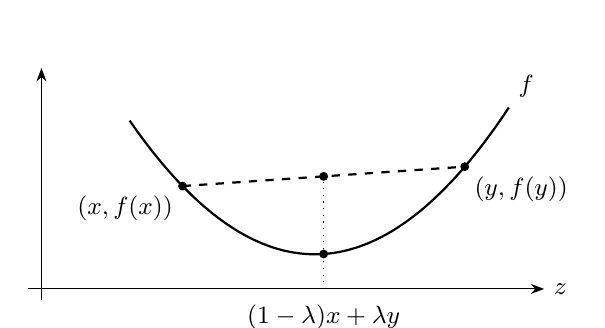
\begin{tikzpicture}[x=1.12cm,y=1.1cm,>=Stealth,font=\small]
  \draw[->] (-1.25,0)--(4.6,0) node[right] {$z$};
  \draw[->] (-1.1,-0.13)--(-1.1,2.55);
  \draw[thick,domain=-0.1:4.2,samples=90]
    plot (\x,{0.35*(\x-2)^2+0.4});
  \draw[thick,dashed] (0.5,1.1875)--(3.7,1.4115);
  \fill (0.5,1.1875) circle(1.6pt) node[below left] {$(x,f(x))$};
  \fill (3.7,1.4115) circle(1.6pt) node[below right] {$(y,f(y))$};
  \draw[dotted] (2.1,0)--(2.1,1.2995);
  \fill (2.1,0.4035) circle(1.6pt);
  \fill (2.1,1.2995) circle(1.6pt);
  \node[below,align=center] at (2.1,-0.07) {$(1-\lambda)x+\lambda y$};
  \node[above right] at (4.2,2.094) {$f$};
\end{tikzpicture}
\end{center}

\QU Which of the following functions are convex on $\R$?
\[
  f_1(x)=x^2,\quad f_2(x)=|x|,\quad
  f_3(x)=3x+1,\quad f_4(x)=-x^2.
\]
\begin{enumerate}
  \aitem Only $f_1$.
  \bitem Only $f_1$ and $f_2$.
  \citem $f_1$, $f_2$, and $f_3$.
  \ditem All four functions.
\end{enumerate}
\end{Qu}
% Answer: C.
\begin{answer}
\textbf{Answer: C.} Convex functions need not be differentiable: $|x|$ has a
corner at $0$. Linear functions satisfy the convexity inequality with
equality. For $-x^2$, take $x=-1$, $y=1$, and $\lambda=1/2$:
the proposed inequality would be $0\leq-1$.
\end{answer}

% ======================== PAGE 5 ========================
\newpage
\subsection{A Second View: Convex Functions Lie Above Their Tangents}

If $f$ is differentiable, its linear, or \textbf{Euler}, approximation at
$x$ is
\[
  f(x)+f'(x)(y-x).
\]
For a general function, this is only a local approximation. For a convex
function, it gives a \hide{global lower bound}.

\begin{lemma}[First-order inequality]\label{lem:convexity}
If $f:\R\to\R$ is differentiable and convex, then, for all $x,y\in\R$,
\[
  \boxed{f(y)\geq f(x)+f'(x)(y-x).}
\]
\end{lemma}

\begin{proof}
For $0<\lambda\leq1$, convexity gives
\[
  f(x+\lambda(y-x))\leq(1-\lambda)f(x)+\lambda f(y).
\]
Rearrange, dividing by the positive number $\lambda$:
\[
  f(y)\geq f(x)+\frac{f(x+\lambda(y-x))-f(x)}{\lambda}.
\]
Let $\lambda\to0^+$. The quotient tends to
\hide{$f'(x)(y-x)$}, which proves the inequality.
\end{proof}

\vs{0.2in}
\textbf{Two compatible pictures of convexity:}
\[
  \text{below every \hide{chord}}
  \qquad\text{and}\qquad
  \text{above every \hide{tangent}}.
\]

\QU Suppose $f$ is differentiable and convex, and $f'(x)=0$.
What can we conclude?
\begin{enumerate}
  \aitem $x$ is necessarily the unique minimizer.
  \bitem $x$ is a global minimizer, but need not be unique.
  \citem $x$ could be a strict local maximum.
  \ditem Nothing about optimality.
\end{enumerate}
\end{Qu}
% Answer: B.
\begin{answer}
\textbf{Answer: B.} For every $y$, the first-order inequality yields
$f(y)\geq f(x)+0\cdot(y-x)=f(x)$. A constant function shows that the
minimizer need not be unique.
\end{answer}

% ======================== PAGE 6 ========================
\newpage
\subsection{Why Local Information Is Useful}

\begin{lemma}[Local minima are global minima]
For a convex function, every local minimum is a global minimum.
\end{lemma}
\begin{proof}
Suppose $x$ is a local minimum but $f(y)<f(x)$ for some $y$.
For sufficiently small $\lambda>0$, the point
$z=(1-\lambda)x+\lambda y$ lies in the neighborhood where $x$ is a minimum.
But
\[
  f(z)\leq(1-\lambda)f(x)+\lambda f(y)<f(x),
\]
which is a contradiction. This argument does not require differentiability.
\end{proof}

\paragraph{The derivative points toward improvement.}
Let $\xstar$ be a minimizer. If $f'(x)>0$, then, for every $y>x$,
\[
  f(y)\geq f(x)+f'(x)(y-x)>f(x).
\]
Thus no minimizer lies to the \hide{right} of $x$. Similarly, if
$f'(x)<0$, no minimizer lies to the \hide{left} of $x$.
Given an interval containing a minimizer, these tests permit binary search.
If $f'(x)=0$, we have already found a global minimizer.

\begin{fact}[Calculus test]
For twice-differentiable $f:\R\to\R$, convexity is equivalent to
$f''(x)\geq0$ for all $x$. Equivalently, $f'$ is nondecreasing.
\end{fact}

\section{Gradient Descent: Move Instead of Discard}

A one-dimensional interval has a natural left and right. In high dimensions,
there is no direct analogue of this interval-based binary search.
An alternative is to move our current point using its derivative:
\[
  \boxed{x_{t+1}=x_t-\eta f'(x_t).}
\]
This is \hide{\textbf{gradient descent}}. The parameter $\eta>0$ is the
\hide{\textbf{step size}}.

\textbf{The design question:} How should we choose $\eta$? Too small may
mean very slow progress; too large may overshoot the minimizer and even
increase the objective. Moving in a descent direction is not, by itself,
a guarantee that an arbitrary-length step decreases $f$.

% ======================== PAGE 7 ========================
\newpage
\section{Smoothness: How Far Can We Safely Move?}

We need a condition that prevents the derivative from changing too quickly.
First, recall a related condition on function values.

\begin{definition}
Let $G\geq0$ and $L>0$. A function $f:\R\to\R$ is
\textbf{$G$-Lipschitz} if, for all $x,y\in\R$,
\[
  |f(x)-f(y)|\leq G|x-y|.
\]
A differentiable function $f:\R\to\R$ is \textbf{$L$-smooth} if, for all
$x,y\in\R$,
\[
  \boxed{|f'(x)-f'(y)|\leq L|x-y|.}
\]
\end{definition}

Lipschitzness of $f$ controls its \hide{values}; smoothness controls its
\hide{derivative}. We use $G$ and $L$ to distinguish these two bounds.

\textbf{Useful calculus tests.} On $\R$, for differentiable $f$,
$|f'|\leq G$ everywhere is equivalent to $G$-Lipschitzness.
For twice-differentiable $f$, $|f''|\leq L$ everywhere is equivalent to
$L$-smoothness.

\QU Classify each function on \emph{all of $\R$}.
\begin{center}
\renewcommand{\arraystretch}{1.35}
\begin{tabular}{lccc}
 & \textbf{Convex?} & \textbf{Lipschitz?} & \textbf{Smooth?}\\\hline
$x^2$ & \hide{Yes} & \hide{No} & \hide{Yes, $L=2$}\\
$|x|$ & \hide{Yes} & \hide{Yes, $G=1$} & \hide{No}\\
$\cos x$ & \hide{No} & \hide{Yes, $G=1$} & \hide{Yes, $L=1$}
\end{tabular}
\end{center}
\end{Qu}

\paragraph{What about simulating derivative queries?}
For $L$-smooth $f$ and $\delta>0$, the fundamental theorem of calculus gives
\begin{align*}
 \left|\frac{f(x+\delta)-f(x)}{\delta}-f'(x)\right|
 &\leq\frac{1}{\delta}\int_0^\delta|f'(x+s)-f'(x)|\,ds\\
 &\leq\frac{1}{\delta}\int_0^\delta Ls\,ds
 =\frac{L\delta}{2}.
\end{align*}
This is an \emph{approximation}, not an exact simulation. Our theorems use
exact derivative queries; finite-difference and floating-point errors are
not included in those guarantees.

% ======================== PAGE 8 ========================
\newpage
\section{Gradient Descent, Take 1: Quadratics}

The simplest smooth convex functions are quadratics. Let
\[
  q(x)=ax^2+bx+c,\qquad a>0.
\]
We can analyze gradient descent exactly in this case.

\paragraph{Where is the minimizer?}
Complete the square:
\begin{align*}
  q(x)
  &=a\left(x+\frac{b}{2a}\right)^2+c-\frac{b^2}{4a},\\[4pt]
  \xstar&=\hide{-\frac{b}{2a}}.
\end{align*}
The additive constant does not affect the location of the minimizer.
The error in the objective value is
\[
  q(x)-q(\xstar)=\hide{a(x-\xstar)^2}.
\]

\paragraph{What does the derivative tell us?}
\[
  q'(x)=2ax+b=\hide{2a(x-\xstar)}.
\]
Thus the derivative is exactly proportional to the signed distance from
the current point to the minimizer. Moreover,
\[
  |q'(x)-q'(y)|=2a|x-y|,
\]
so the tight smoothness constant is \hide{$L=2a$}.

\begin{example}\textbf{Complete the Square}
Let $q(x)=x^2-6x+10$. Find the minimizer, the minimum value, the derivative,
and a tight smoothness constant.
\end{example}
\begin{answer}
\begin{align*}
  q(x)&=(x-3)^2+1,&\xstar&=3,\\
  q(\xstar)&=1,&q'(x)&=2x-6,\qquad L=2.
\end{align*}
\end{answer}
\vs{0.4in}

\textbf{Next question:} Can we choose a step size that lands directly at
$\xstar$?

% ======================== PAGE 9 ========================
\newpage
\subsection{Choosing and Testing the Step Size}

For a quadratic with tight smoothness constant $L=2a$, a gradient step is
\[
  x_{t+1}=x_t-\eta L(x_t-\xstar).
\]
Subtracting $\xstar$ from both sides gives the exact recurrence
\[
  \boxed{x_{t+1}-\xstar=(1-\eta L)(x_t-\xstar).}
\]
With $\eta=\hide{1/L}$, the multiplier is zero: we reach the minimizer in
\hide{one step}. A larger valid upper bound on smoothness gives a smaller,
still safe step, but need not give one-step convergence.

\begin{example}\textbf{Trace the Iterates}
Use $q(x)=x^2-6x+10$, $x_0=0$, and $L=2$. Compute $x_1$ and $x_2$ for each
choice of $\eta$.
\begin{center}
\renewcommand{\arraystretch}{1.6}
\begin{tabular}{c|cc|l}
$\eta$ & $x_1$ & $x_2$ & \textbf{Behavior}\\\hline
$1/4$ & \hide{$3/2$} & \hide{$9/4$} & \hide{Approaches from one side}\\
$1/2$ & \hide{$3$} & \hide{$3$} & \hide{Reaches the minimizer}\\
$3/4$ & \hide{$9/2$} & \hide{$9/4$} & \hide{Alternates, but gets closer}\\
$1$ & \hide{$6$} & \hide{$0$} & \hide{Oscillates without progress}
\end{tabular}
\end{center}
\end{example}

\QU Does overshooting always imply that gradient descent diverges?
Use the recurrence to determine exactly when the distance decreases
for this quadratic.
\end{Qu}
\begin{answer}
No. The distance decreases at every nonoptimal iterate precisely when
\[
  |1-\eta L|<1\quad\Longleftrightarrow\quad 0<\eta<\frac{2}{L}.
\]
For $1/L<\eta<2/L$, the iterates cross the minimizer but get closer.
At $\eta=2/L$, a nonoptimal starting point oscillates. For $\eta>2/L$, its
distance grows. Thus $1/L$ is a convenient safe choice, not the only
convergent choice for a quadratic.
\end{answer}
\vs{0.15in}

\textbf{Progress with $\eta=1/L$:}
\[
  q(x)-q\left(x-\frac{q'(x)}{L}\right)
  =a(x-\xstar)^2=\hide{\frac{(q'(x))^2}{2L}}.
\]

% ======================== PAGE 10 ========================
\newpage
\section{Gradient Descent, Take 2: Smooth Functions}

A general smooth function is not a quadratic. The useful replacement is
that it has a \textbf{quadratic upper bound} centered at every point.

\begin{lemma}[Quadratic upper bound]\label{lem:smooth}
If $f:\R\to\R$ is $L$-smooth, then, for every $x,y\in\R$,
\[
  \boxed{f(y)\leq f(x)+f'(x)(y-x)+\frac L2(y-x)^2.}
\]
Convexity is \emph{not} required.
\end{lemma}

\textbf{Intuition.} A first-order approximation uses the tangent line.
Smoothness controls how far the derivative can move away from its initial
value, so the error accumulated along a step is at most quadratic in the
step length.

\begin{proof}
Write $h=y-x$. Parameterizing the segment from $x$ to $y$ by $x+sh$, where
$0\leq s\leq1$, gives
\begin{align*}
 f(y)-f(x)-f'(x)h
   &=\int_0^1\bigl(f'(x+sh)-f'(x)\bigr)h\,ds\\
   &\leq\int_0^1|f'(x+sh)-f'(x)|\,|h|\,ds\\
   &\leq\int_0^1 Ls|h|^2\,ds\\
   &=\hide{\frac L2 h^2}.
\end{align*}
The absolute values make the argument valid whether $y\geq x$ or $y<x$.
Substitute $h=y-x$ and rearrange.
\end{proof}

\vs{0.25in}
For a function that is \emph{both convex and $L$-smooth}, we now have
\begin{align*}
  f(x)+f'(x)(y-x)
  &\leq f(y)\\
  &\leq f(x)+f'(x)(y-x)+\frac L2(y-x)^2.
\end{align*}
Convexity supplies the \hide{linear lower bound}.\\
Smoothness supplies the \hide{quadratic upper bound}.\\
These two inequalities play different roles in the analysis.

% ======================== PAGE 11 ========================
\newpage
\subsection{Minimize the Upper Bound, Not the Unknown Function}

At the current point $x$, define the quadratic model
\[
  Q_x(y)=f(x)+f'(x)(y-x)+\frac L2(y-x)^2.
\]
We know $Q_x(x)=f(x)$ and $f(y)\leq Q_x(y)$ for all $y$.

\begin{center}
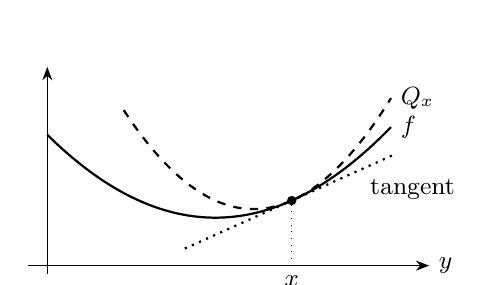
\begin{tikzpicture}[x=0.97cm,y=0.87cm,>=Stealth,font=\small]
  \draw[->] (-2.45,0)--(2.8,0) node[right] {$y$};
  \draw[->] (-2.2,-0.12)--(-2.2,2.9);
  % f(y)=0.25*y^2+0.7, anchor x=1, and a valid L=1 upper model.
  \draw[thick,domain=-2.2:2.3,samples=90]
    plot (\x,{0.25*(\x)^2+0.7});
  \draw[dashed,thick,domain=-1.2:2.3,samples=90]
    plot (\x,{0.95+0.5*(\x-1)+0.5*(\x-1)^2});
  \draw[dotted,thick] (-0.4,0.25)--(2.35,1.625);
  \fill (1,0.95) circle(1.7pt);
  \draw[dotted] (1,0)--(1,0.95);
  \node[below] at (1,0) {$x$};
  \node[right] at (2.3,2.445) {$Q_x$};
  \node[right] at (2.3,2.0225) {$f$};
  \node[below right] at (1.9,1.4) {tangent};
\end{tikzpicture}
\end{center}

Differentiate the quadratic model with respect to $y$:
\[
  Q_x'(y)=f'(x)+L(y-x).
\]
Setting this equal to zero gives its minimizer
\[
  y=\hide{x-\frac{f'(x)}{L}}.
\]
Thus gradient descent with $\eta=1/L$ minimizes a valid quadratic upper
bound at every iteration.

\begin{lemma}[One-step progress]\label{lem:descent}
For any $L$-smooth $f$, the point $x^+=x-f'(x)/L$ satisfies
\[
  \boxed{f(x^+)\leq f(x)-\frac{(f'(x))^2}{2L}.}
\]
\end{lemma}
\begin{proof}
Substitute $y=x-f'(x)/L$ into Lemma~\ref{lem:smooth}:
\[
 f(x^+)\leq f(x)-\frac{(f'(x))^2}{L}
              +\frac{L}{2}\frac{(f'(x))^2}{L^2}
          =f(x)-\frac{(f'(x))^2}{2L}.
\]
\end{proof}

% ======================== PAGE 12 ========================
\newpage
\section{The Algorithm and Its Two Possible Guarantees}

\begin{algorithm}[H]
\caption{Gradient-Descent$(f,x_0,L,T)$}\label{alg:gd}
\begin{algorithmic}[1]
  \Require Derivative access to an $L$-smooth function $f:\R\to\R$;
     $L>0$; initial point $x_0$; integer $T\geq1$
  \State $g_{\mathrm{best}}\gets+\infty$
  \For{$t=0,1,\ldots,T-1$}
    \State $g_t\gets f'(x_t)$
    \If{$|g_t|<g_{\mathrm{best}}$}
      \State $\widehat x\gets x_t$; $g_{\mathrm{best}}\gets |g_t|$
    \EndIf
    \State $x_{t+1}\gets x_t-g_t/L$
  \EndFor
  \State \Return $x_T$ and $\widehat x$
\end{algorithmic}
\end{algorithm}

\textbf{Which output?} We use $\widehat x$ for a small-derivative guarantee,
and $x_T$ for the convex objective-value guarantee. There is no need to
store all previous iterates: retaining the current point and the best
observed derivative magnitude is enough.

\textbf{Runtime.} The algorithm makes \hide{$T$} derivative queries.
If one derivative costs $C_{\mathrm{grad}}$ time, the total time is
\hide{$O(T(C_{\mathrm{grad}}+1))$} in the real-arithmetic model.

\begin{definition}
A point $x$ is an \textbf{$\eps$-critical point} if $|f'(x)|\leq\eps$.
A point $x$ is an \textbf{$\eps$-approximate minimizer} if
$f(x)-f(\xstar)\leq\eps$.
\end{definition}

These are \textbf{different guarantees}. Smoothness alone will let us find
an approximate critical point. Convexity and a distance bound will connect
criticality to global optimality.

\QU Let $f(x)=\cos x$. Gradient descent starts at $x_0=0$.
What happens, and is the output a local minimum?
\end{Qu}
\begin{answer}
Since $f'(0)=-\sin0=0$, every iterate remains at $0$.
But $f(0)=1$ is a global maximum, while $f(\pi)=-1$.
The function is $1$-smooth. Thus even an exactly critical point need not
be a local minimum of a smooth, nonconvex function.
\end{answer}
\vs{0.2in}

\textbf{Scope reminder.} We are minimizing over $\R$. At the boundary of a
constrained feasible set, an optimum need not have derivative zero.

% ======================== PAGE 13 ========================
\newpage
\section{Analysis I: Finding an Approximate Critical Point}

\begin{theorem}[Smooth, possibly nonconvex objective]\label{thm:critical}
Let $f:\R\to\R$ be $L$-smooth, with a minimizer $\xstar$, and suppose $\Delta\geq0$ satisfies
\[
  f(x_0)-f(\xstar)\leq\Delta.
\]
After $T\geq1$ iterations of Algorithm~\ref{alg:gd},
\[
  \boxed{\min_{0\leq t<T}|f'(x_t)|
          \leq\sqrt{\frac{2L\Delta}{T}}.}
\]
In particular, $T\geq 2L\Delta/\eps^2$ suffices for the returned
$\widehat x$ to be an $\eps$-critical point.
\end{theorem}

\textbf{Proof idea.} A large derivative forces a substantial decrease in
$f$. But the total decrease cannot exceed the initial gap $\Delta$.

\begin{proof}
By Lemma~\ref{lem:descent}, for every $0\leq t<T$,
\[
  \frac{(f'(x_t))^2}{2L}\leq f(x_t)-f(x_{t+1}).
\]
Sum over the $T$ iterations. The right-hand side telescopes:
\begin{align*}
  \frac{1}{2L}\sum_{t=0}^{T-1}(f'(x_t))^2
  &\leq f(x_0)-f(x_T)\\
  &\leq f(x_0)-f(\xstar)\leq\Delta.
\end{align*}
The smallest squared derivative is at most their average, so
\[
  \min_{0\leq t<T}(f'(x_t))^2
   \leq\frac1T\sum_{t=0}^{T-1}(f'(x_t))^2
   \leq\hide{\frac{2L\Delta}{T}}.
\]
Taking square roots proves the result.
\end{proof}

\QU Holding $L$ and $\Delta$ fixed, how does the sufficient iteration count
change if the desired derivative tolerance decreases from $\eps$ to
$\eps/2$?
\end{Qu}
\begin{answer}
It increases by a factor of $4$, since the bound is proportional to
$1/\eps^2$. Notice that no part of the proof used convexity.
\end{answer}

% ======================== PAGE 14 ========================
\newpage
\section{Analysis II: Adding Convexity}

For a convex objective, Lemma~\ref{lem:convexity} gives
\begin{align*}
 f(x)-f(\xstar)
 &\leq f'(x)(x-\xstar)\\
 &\leq |f'(x)|\,|x-\xstar|.
\end{align*}
A small derivative therefore gives a small objective gap \emph{provided}
we also control the distance to a minimizer.

\begin{lemma}[Distance never increases]\label{lem:distance}
Let $f:\R\to\R$ be convex and $L$-smooth, with minimizer $\xstar$.
For $x^+=x-f'(x)/L$,
\[
  |x^+-\xstar|\leq |x-\xstar|.
\]
Consequently, if $|x_0-\xstar|\leq R$, then $|x_t-\xstar|\leq R$
for every gradient-descent iterate.
\end{lemma}

\begin{proof}
Write $g=f'(x)$. Expanding the squared distance gives
\[
 (x^+-\xstar)^2
  =(x-\xstar)^2-\frac{2}{L}g(x-\xstar)+\frac{g^2}{L^2}.
\]
We need $g(x-\xstar)\geq g^2/(2L)$. To prove this, chain together
three facts:
\begin{align*}
  g(x-\xstar)
  &\geq f(x)-f(\xstar) &&\text{by convexity}\\
  &\geq f(x)-f(x^+) &&\text{by optimality of }\xstar\\
  &\geq \frac{g^2}{2L} &&\text{by one-step progress}.
\end{align*}
Substituting yields
\[
 (x^+-\xstar)^2
 \leq(x-\xstar)^2
   -\frac{2}{L}\frac{g^2}{2L}+\frac{g^2}{L^2}
 =(x-\xstar)^2.
\]
Both distances are nonnegative, so taking square roots proves the
one-step claim. Apply it repeatedly to obtain the statement for every $t$.
\end{proof}

\textbf{What to remember:} Smoothness controls how much a step can change
$f$; convexity supplies the inequality that also controls the distance.

% ======================== PAGE 15 ========================
\newpage
\subsection{A First Global Convergence Guarantee}

\begin{theorem}[Introductory convex guarantee]\label{thm:global}
Suppose $f:\R\to\R$ is convex and $L$-smooth, attains its minimum at
$\xstar$, and $|x_0-\xstar|\leq R$, where $R>0$. For every $T\geq1$,
Algorithm~\ref{alg:gd} satisfies
\[
  \boxed{f(x_T)-f(\xstar)\leq\frac{LR^2}{\sqrt T}.}
\]
Hence $T\geq L^2R^4/\eps^2$ suffices for an $\eps$-approximate minimizer.
\end{theorem}

\textbf{Proof idea.} Bound the initial objective gap, find a small
derivative, and use convexity together with the distance invariant.

\begin{proof}
\textbf{Step 1: Bound the initial gap.}
Since $\xstar$ is an unconstrained minimizer of a differentiable function,
$f'(\xstar)=0$. Center Lemma~\ref{lem:smooth} at $\xstar$:
\[
  f(x_0)-f(\xstar)
  \leq \frac L2(x_0-\xstar)^2
  \leq\frac{LR^2}{2}.
\]
Thus we may use $\Delta=LR^2/2$ in Theorem~\ref{thm:critical}.

\textbf{Step 2: Find an iterate with a small derivative.}
For some $0\leq t<T$,
\[
  |f'(x_t)|\leq\sqrt{\frac{2L\Delta}{T}}
          =\frac{LR}{\sqrt T}.
\]

\textbf{Step 3: Convert criticality to global optimality.}
Convexity and Lemma~\ref{lem:distance} imply
\[
  f(x_t)-f(\xstar)
  \leq |f'(x_t)|\,|x_t-\xstar|
  \leq \frac{LR}{\sqrt T}\,R=\frac{LR^2}{\sqrt T}.
\]
Finally, Lemma~\ref{lem:descent} says the objective values never increase.
Since $t<T$, we have $f(x_T)\leq f(x_t)$, which proves the claim for the
\emph{last} iterate.
\end{proof}

\textbf{Equivalent accuracy calculation.} To make the objective gap at
most $\eps$, it suffices to find a derivative of magnitude $\eps/R$:
\[
  \frac{2L(LR^2/2)}{(\eps/R)^2}
  =\hide{\frac{L^2R^4}{\eps^2}}\quad\text{iterations suffice.}
\]

% ======================== PAGE 16 ========================
\newpage
\section{The Higher-Dimensional Viewpoint}

Now let $x=(x_1,\ldots,x_d)\in\R^d$. A set $\X\subseteq\R^d$ is
\textbf{convex} if it contains the entire line segment between every pair
of its points:
\[
  x,y\in\X,\ \lambda\in[0,1]
  \quad\Longrightarrow\quad (1-\lambda)x+\lambda y\in\X.
\]
A function $f:\X\to\R$ is convex if $\X$ is convex and
\[
 f((1-\lambda)x+\lambda y)
 \leq (1-\lambda)f(x)+\lambda f(y).
\]
Minimizing a convex function over a convex set is a
\hide{\textbf{convex optimization problem}}. Our gradient-descent analysis
concerns the unconstrained case $\X=\R^d$.

\paragraph{Replace the derivative with a gradient.}
For differentiable $f:\R^d\to\R$, the gradient is
\[
 \nabla f(x)=\begin{pmatrix}
  \partial f(x)/\partial x_1\\
  \vdots\\
  \partial f(x)/\partial x_d
 \end{pmatrix}.
\]
Write $\langle u,v\rangle=\sum_i u_iv_i$ and
$\|u\|_2=\sqrt{\sum_i u_i^2}$.
Euclidean $L$-smoothness means
\[
  \|\nabla f(x)-\nabla f(y)\|_2\leq L\|x-y\|_2.
\]
The update becomes
\[
  \boxed{x_{t+1}=x_t-\frac1L\nabla f(x_t).}
\]

\begin{example}\textbf{A Two-Dimensional Step}
Let $f(u,v)=u^2+4v^2$. Verify that $L=8$ is valid, and take one gradient
descent step from $(2,1)$ with $\eta=1/8$.
\end{example}
\begin{answer}
The gradient is $(2u,8v)$, and
$\|(2a,8b)\|_2^2=4a^2+64b^2\leq64(a^2+b^2)$.
At $(2,1)$, the gradient is $(4,8)$, so the next point is
$(2,1)-(4,8)/8=(3/2,0)$. A single step size need not solve both
coordinates in one step.
\end{answer}

% ======================== PAGE 17 ========================
\newpage
\subsection{The Same Analysis, With Inner Products and Norms}

The two central inequalities generalize to
\begin{align*}
 f(y)&\geq f(x)+\langle\nabla f(x),y-x\rangle
          &&\text{(convexity)},\\
 f(y)&\leq f(x)+\langle\nabla f(x),y-x\rangle
                  +\frac L2\|y-x\|_2^2
          &&\text{(smoothness)}.
\end{align*}
In particular, the same substitution into the upper bound gives
\[
 f\left(x-\frac1L\nabla f(x)\right)
 \leq f(x)-\frac{\|\nabla f(x)\|_2^2}{2L}.
\]
The telescoping proof therefore gives
\[
  \min_{0\leq t<T}\|\nabla f(x_t)\|_2
  \leq\sqrt{\frac{2L\Delta}{T}}.
\]
For the convex guarantee, replace squared scalar distances by squared
Euclidean distances in Lemma~\ref{lem:distance}, and use Cauchy--Schwarz:
\[
  f(x)-f(\xstar)
  \leq\langle\nabla f(x),x-\xstar\rangle
  \leq\|\nabla f(x)\|_2\,\|x-\xstar\|_2.
\]
Thus the introductory bound in Theorem~\ref{thm:global} also holds when
$\|x_0-\xstar\|_2\leq R$.

\textbf{Iterations are not the same as runtime.} There is no explicit $d$
in these iteration bounds. However, $L$, $R$, and the cost of a gradient
can depend on $d$. Each vector update also takes $O(d)$ arithmetic
operations, so $T$ iterations cost
\[
  O\bigl(T(C_{\mathrm{grad}}+d)\bigr).
\]

\QU Which statement is justified by today's analysis?
\begin{enumerate}
  \aitem A small gradient always means a nearby minimizer.
  \bitem Smoothness alone guarantees a global minimum.
  \citem A constant number of scalar arithmetic operations always suffices
  for one iteration, regardless of $d$.
  \ditem Smoothness guarantees progress proportional to the squared
  gradient norm; convexity can turn local information into a global bound.
\end{enumerate}
\end{Qu}
% Answer: D.
\begin{answer}
\textbf{Answer: D.} A confuses derivative size with distance to a
minimizer; B assumes smoothness implies global optimality; C ignores the
cost of processing $d$ coordinates.
\end{answer}

% ======================== PAGE 18 ========================
\newpage
\section{Summary and Beyond Today's Analysis}

\paragraph{The algorithm.}
Start from $x_0$ and repeatedly use the local slope to improve the current
guess. In one dimension,
\[
  x_{t+1}=x_t-\frac1L f'(x_t).
\]
In $\R^d$, replace $f'(x_t)$ with $\nabla f(x_t)$.

\paragraph{The role of each assumption.}
\textbf{Smoothness} gives a quadratic upper bound and a safe step size.
\textbf{Convexity} gives a linear lower bound and rules out nonglobal local
minima. A bound on the initial gap or distance turns these structural
statements into an iteration count.

\paragraph{The guarantees proved in this lecture.}
For a smooth objective with initial value gap at most $\Delta$,
\[
  T\geq\frac{2L\Delta}{\eps^2}
  \quad\Longrightarrow\quad
  \text{an $\eps$-critical point among the queried iterates}.
\]
For a smooth convex objective with initial distance at most $R$,
\[
  T\geq\frac{L^2R^4}{\eps^2}
  \quad\Longrightarrow\quad
  f(x_T)-f(\xstar)\leq\eps.
\]
Take the ceiling of the displayed iteration bound, and at least one
iteration. These results assume an attained optimum and exact gradients.

\paragraph{Stronger results: stated, not proved here.}
The supplied notes, Section 2.4, point out that a sharper analysis of the
\emph{same} gradient-descent algorithm gives an $\eps$-approximate minimizer
in $O(LR^2/\eps)$ iterations. The $1/\eps^2$ dependence above is a limitation
of our introductory proof, not the best bound for gradient descent.

The notes also describe \textbf{acceleration}: an appropriately modified
algorithm using momentum attains $O(\sqrt{LR^2/\eps})$ iterations for smooth
convex minimization. Arbitrarily adding momentum does not inherit this
guarantee; the method and its analysis are beyond today's lecture.

\paragraph{Sources.}
Kevin Tian, \emph{CS331, Part VI: Continuous Algorithms}, Sections 1--2
(especially Lemmas 1--5) and Section 5.1; and \emph{CS331, Fall 2025,
Lecture 15 (10/20)}. These sources supply the theory and lecture sequence.
Exercises and questions were written for this adaptation.

\end{document}
'
%
% Source scope: Part6_main.pdf, Sections 1--2 (main lecture), and
% Section 5.1 (definition of a convex set in the final extension).
% The companion 10-20.pdf supplies the one-dimensional-first progression.
% New numerical examples and questions are practice exercises, not quotations.

\documentclass[11pt,letterpaper]{article}
\usepackage[lmargin=1in,rmargin=1.75in,bmargin=1in,tmargin=1in]{geometry}
\usepackage[T1]{fontenc}
\usepackage{lmodern}
\usepackage{amsmath,amssymb,amsthm}
\usepackage{graphicx}
\usepackage{setspace}
\usepackage{enumitem}
\usepackage{algorithm}
\usepackage{algpseudocode}
\usepackage{float}
\usepackage{tikz}
\usepackage{environ}
\usepackage{fancyhdr}
\usepackage{microtype}
\usepackage[hidelinks]{hyperref}
\usetikzlibrary{arrows.meta}

% ---------------- Editable course information ----------------
\newcommand{\CourseName}{CSCE 411: Design and Analysis of Algorithms}
\newcommand{\LectureDate}{} % Fill in the actual lecture date here.
\newcommand{\LectureNumber}{} % Optional, e.g., 15: (include the colon).

% ---------------- Standalone course-style definitions ----------------
\newif\ifstudentversion
\studentversionfalse
\ifdefined\studenthandout\studentversiontrue\fi
\newcommand{\vs}[1]{\vspace{#1}}
\newcommand{\hide}[1]{%
  \ifstudentversion
    \ifmmode\phantom{#1}\else\underline{\phantom{#1}}\fi
  \else #1\fi}
\newcommand{\lecture}[2]{%
  \noindent\textbf{\CourseName}\hfill #2\par
  \vspace{5pt}\hrule\vspace{10pt}
  {\centering\Large\bfseries #1\par}
  \vspace{10pt}\hrule\vspace{9pt}}
\theoremstyle{definition}
\newtheorem{definition}{Definition}
\newtheorem{example}{Example}
\theoremstyle{plain}
\newtheorem{lemma}{Lemma}
\newtheorem{theorem}{Theorem}
\newtheorem{fact}{Fact}
\newcounter{question}
\newenvironment{Qu}{%
  \par\medskip\refstepcounter{question}
  \noindent\textbf{Question \thequestion.}\ }{\par\medskip}
\newcommand{\QU}{\begin{Qu}}
\newcommand{\aitem}{\item[\textbf{(A)}]}
\newcommand{\bitem}{\item[\textbf{(B)}]}
\newcommand{\citem}{\item[\textbf{(C)}]}
\newcommand{\ditem}{\item[\textbf{(D)}]}
\newcommand{\eitem}{\item[\textbf{(E)}]}
\newsavebox{\answerbox}
% Answers occupy the same space in both versions; in the student version
% this space is left blank for the in-class calculation or discussion.
\NewEnviron{answer}{%
  \par\begingroup
  \setbox\answerbox=\vbox{\hsize=\linewidth\parindent=0pt\BODY\par}%
  \noindent\ifstudentversion\phantom{\usebox{\answerbox}}%
  \else\usebox{\answerbox}\fi\par\endgroup}
\newenvironment{problemframe}{%
  \par\smallskip\noindent
  \begin{lrbox}{\answerbox}
  \begin{minipage}{\dimexpr\linewidth-2\fboxsep-2\fboxrule\relax}}%
  {\end{minipage}\end{lrbox}\fbox{\usebox{\answerbox}}\par\smallskip}
\newcommand{\R}{\mathbb R}
\newcommand{\X}{\mathcal X}
\newcommand{\eps}{\varepsilon}
\newcommand{\xstar}{x^\star}
\DeclareMathOperator*{\argmin}{arg\,min}
\setlength{\parindent}{0pt}
\setlength{\parskip}{5pt}
\setlength{\headheight}{14pt}
\setlist[itemize]{topsep=3pt,itemsep=2pt,parsep=0pt}
\setlist[enumerate]{topsep=3pt,itemsep=2pt,parsep=0pt,leftmargin=2.1em}
\pagestyle{fancy}
\fancyhf{}
\fancyhead[L]{\small Convex Optimization and Gradient Descent}
\fancyhead[R]{\small CSCE 411}
\fancyfoot[C]{\thepage}
\renewcommand{\headrulewidth}{0.3pt}
\renewcommand{\footrulewidth}{0pt}
\raggedbottom
\hypersetup{pdftitle={Introduction to Convex Optimization and Gradient Descent},
  pdfauthor={CSCE 411 Lecture Notes},pdfsubject={Design and Analysis of Algorithms}}

\begin{document}
\onehalfspacing
\thispagestyle{plain}

% ======================== PAGE 1 ========================
\lecture{\LectureNumber\ Introduction to Convex Optimization\\and Gradient Descent}{\LectureDate}

\paragraph{Reading.}
Kevin Tian, \emph{Part VI: Continuous Algorithms}, Sections 1--2;
and the accompanying October 20 lecture notes. The last section briefly
introduces the higher-dimensional viewpoint from Section 5.1.

\section{Motivation: From Discrete to Continuous Optimization}

Many problems we have studied ask us to choose the best object from a set of
possible objects. We can write this common form as
\[
  \min_{x\in\X} f(x)
  \qquad\text{or}\qquad
  \max_{x\in\X} f(x).
\]
The variable $x$ is the \hide{\textbf{decision variable}}, the set $\X$ is the
\hide{\textbf{feasible set}}, and $f$ is the \hide{\textbf{objective function}}.

\begin{center}
\renewcommand{\arraystretch}{1.25}
\begin{tabular}{lll}
\textbf{Problem} & \textbf{Feasible objects} & \textbf{Objective}\\\hline
Interval scheduling & Nonoverlapping subsets & Maximize subset size\\
Minimum spanning tree & Spanning trees & Minimize total weight\\
Shortest path & $s$--$t$ paths & Minimize total weight
\end{tabular}
\end{center}

In these examples, the choices are discrete. Today, the decision variable
can instead be a real number or a vector of real numbers: $x\in\X\subseteq\R^d$.
There may be infinitely many feasible choices!

\begin{example}\textbf{Approximate Continuous Minimization}
\begin{problemframe}
\textbf{Input:} A function $f:\X\to\R$, a nonempty feasible set
$\X\subseteq\R^d$, and an accuracy parameter $\eps>0$.

\textbf{Output:} A point $\widehat x\in\X$ satisfying
\[
  f(\widehat x)\leq \hide{f(\xstar)+\eps},
  \qquad \xstar\in\argmin_{x\in\X} f(x).
\]
Here we assume that a minimizer $\xstar$ exists.
\end{problemframe}
\end{example}

Our accuracy target concerns the \emph{objective value}, not necessarily the
location of the output. An additive error of $\eps$ need not imply
$|\widehat x-\xstar|\leq\eps$.

% ======================== PAGE 2 ========================
\newpage
\subsection{A Familiar Example: Maximum Flow}

A maximum-flow problem already has a continuous formulation. Let
$G=(V,E)$ be a directed graph, with source $s$, sink $t$, and capacities
$c_e\geq0$. For this formulation, assume no edges enter $s$ or leave $t$.
Let $x_e$ denote the flow on edge $e$, so the decision variable is
$x\in\R^{|E|}$.

We want to maximize
\[
  f(x)=\sum_{e=(s,v)\in E}x_e
\]
subject to the constraints
\begin{align*}
  0\leq x_e&\leq c_e &&\text{for every }e\in E,\\
  \sum_{e=(u,v)\in E}x_e&=
  \sum_{e=(v,w)\in E}x_e &&\text{for every }v\in V\setminus\{s,t\}.
\end{align*}
The first constraints enforce \hide{capacity bounds}; the second enforce
\hide{flow conservation}. The feasible set $\X$ contains every flow satisfying
these constraints.

\QU Suppose there is a nonzero feasible flow $x$. Why are there infinitely
many feasible flows, even though the graph is finite?
\end{Qu}
\begin{answer}
For every $\lambda\in[0,1]$, the scaled flow $\lambda x$ is feasible:
capacity inequalities and conservation are preserved. Because $x\neq0$,
different values of $\lambda$ give different flows.
\end{answer}
\vs{0.25in}

\subsection{Another Motivation: Fitting a Model to Data}

Suppose $x\in\R^d$ records the parameters of a prediction rule. We can use a
\textbf{loss function} $f(x)$ to measure its errors on a collection of
training examples, and choose the parameters by minimizing $f(x)$.

There are infinitely many parameter choices, so enumerating all models is
not an option. Instead, we will repeatedly improve a current guess using
local information about the objective.

\textbf{Important distinction.} The loss of a complicated model need not be
convex. Our analysis will separate what smoothness alone guarantees from
what additionally requires convexity.

% ======================== PAGE 3 ========================
\newpage
\section{What Information Can an Algorithm Use?}

In the \hide{\textbf{oracle model}}, we ask for information about $f$ at
points of our choice. A \textbf{value query} returns $f(x)$; a
\textbf{derivative query} returns $f'(x)$ in one dimension.
We count queries separately from the cost of computing them.
For the gradient-descent theorems, we assume exact derivative queries and
exact real arithmetic.

Derivative queries are natural because a derivative describes how the
function changes nearby. Value queries can also \emph{approximate} a
derivative through
\[
  f'(x)\approx\frac{f(x+\delta)-f(x)}{\delta},
  \qquad \delta>0.
\]
We will make the approximation error precise after defining smoothness.

\subsection{Without Structure, Queries May Tell Us Nothing}

For an unknown point $z\in[0,1]$, consider
\[
  f_z(x)=
  \begin{cases}
    0,&x=z,\\
    1,&x\neq z.
  \end{cases}
\]
Even finding $\widehat x$ with $f_z(\widehat x)\leq\min f_z+0.99$ requires
finding \hide{the exact point $z$}.

\textbf{Why finitely many queries cannot guarantee success.}
Consider a deterministic algorithm and answer every query with $1$.
After its finite query sequence and output $\widehat x$, choose $z$ outside
all queried points and outside $\{\widehat x\}$. Every answer is consistent
with $f_z$, but the output has value $1$ while the minimum is $0$.

\textbf{Takeaway:} A bounded domain and bounded function values are not
enough. We need assumptions under which queries provide useful information.

\paragraph{A contrasting example: unimodality.}
If $f$ is strictly decreasing up to a minimizer $c$ and strictly increasing
afterward, compare its values at
\[
  u=\ell+\frac{r-\ell}{3},\qquad
  v=\ell+\frac{2(r-\ell)}{3}
\]
in a known interval $[\ell,r]$ containing $c$. If $f(u)<f(v)$, discard
$(v,r]$; if $f(u)>f(v)$, discard $[\ell,u)$; if they are equal, retain $[u,v]$.
This is \hide{\textbf{ternary search}}: local queries now reveal which
part of the interval can contain the minimizer.

% ======================== PAGE 4 ========================
\newpage
\section{Convexity: Structure That Helps Optimization}

We first work in \textbf{one dimension}. Unless otherwise specified,
$f:\R\to\R$, and we minimize over all of $\R$.

\begin{definition}
A function $f:\R\to\R$ is \hide{\textbf{convex}} if, for every $x,y\in\R$
and every $\lambda\in[0,1]$,
\[
  \boxed{f((1-\lambda)x+\lambda y)
  \leq (1-\lambda)f(x)+\lambda f(y).}
\]
\end{definition}

The point $(1-\lambda)x+\lambda y$ is a weighted average of $x$ and $y$.
The right-hand side is the height of the line segment joining
$(x,f(x))$ and $(y,f(y))$. A convex function lies \hide{at or below}
every such segment.

\begin{center}
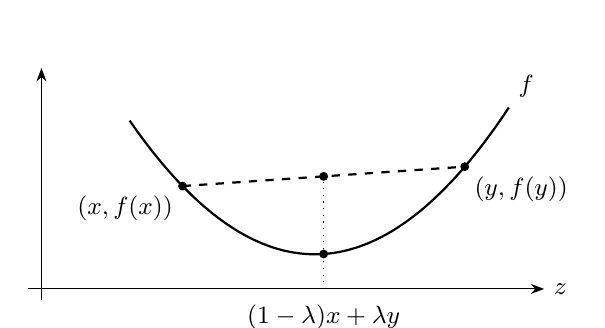
\begin{tikzpicture}[x=1.12cm,y=1.1cm,>=Stealth,font=\small]
  \draw[->] (-1.25,0)--(4.6,0) node[right] {$z$};
  \draw[->] (-1.1,-0.13)--(-1.1,2.55);
  \draw[thick,domain=-0.1:4.2,samples=90]
    plot (\x,{0.35*(\x-2)^2+0.4});
  \draw[thick,dashed] (0.5,1.1875)--(3.7,1.4115);
  \fill (0.5,1.1875) circle(1.6pt) node[below left] {$(x,f(x))$};
  \fill (3.7,1.4115) circle(1.6pt) node[below right] {$(y,f(y))$};
  \draw[dotted] (2.1,0)--(2.1,1.2995);
  \fill (2.1,0.4035) circle(1.6pt);
  \fill (2.1,1.2995) circle(1.6pt);
  \node[below,align=center] at (2.1,-0.07) {$(1-\lambda)x+\lambda y$};
  \node[above right] at (4.2,2.094) {$f$};
\end{tikzpicture}
\end{center}

\QU Which of the following functions are convex on $\R$?
\[
  f_1(x)=x^2,\quad f_2(x)=|x|,\quad
  f_3(x)=3x+1,\quad f_4(x)=-x^2.
\]
\begin{enumerate}
  \aitem Only $f_1$.
  \bitem Only $f_1$ and $f_2$.
  \citem $f_1$, $f_2$, and $f_3$.
  \ditem All four functions.
\end{enumerate}
\end{Qu}
% Answer: C.
\begin{answer}
\textbf{Answer: C.} Convex functions need not be differentiable: $|x|$ has a
corner at $0$. Linear functions satisfy the convexity inequality with
equality. For $-x^2$, take $x=-1$, $y=1$, and $\lambda=1/2$:
the proposed inequality would be $0\leq-1$.
\end{answer}

% ======================== PAGE 5 ========================
\newpage
\subsection{A Second View: Convex Functions Lie Above Their Tangents}

If $f$ is differentiable, its linear, or \textbf{Euler}, approximation at
$x$ is
\[
  f(x)+f'(x)(y-x).
\]
For a general function, this is only a local approximation. For a convex
function, it gives a \hide{global lower bound}.

\begin{lemma}[First-order inequality]\label{lem:convexity}
If $f:\R\to\R$ is differentiable and convex, then, for all $x,y\in\R$,
\[
  \boxed{f(y)\geq f(x)+f'(x)(y-x).}
\]
\end{lemma}

\begin{proof}
For $0<\lambda\leq1$, convexity gives
\[
  f(x+\lambda(y-x))\leq(1-\lambda)f(x)+\lambda f(y).
\]
Rearrange, dividing by the positive number $\lambda$:
\[
  f(y)\geq f(x)+\frac{f(x+\lambda(y-x))-f(x)}{\lambda}.
\]
Let $\lambda\to0^+$. The quotient tends to
\hide{$f'(x)(y-x)$}, which proves the inequality.
\end{proof}

\vs{0.2in}
\textbf{Two compatible pictures of convexity:}
\[
  \text{below every \hide{chord}}
  \qquad\text{and}\qquad
  \text{above every \hide{tangent}}.
\]

\QU Suppose $f$ is differentiable and convex, and $f'(x)=0$.
What can we conclude?
\begin{enumerate}
  \aitem $x$ is necessarily the unique minimizer.
  \bitem $x$ is a global minimizer, but need not be unique.
  \citem $x$ could be a strict local maximum.
  \ditem Nothing about optimality.
\end{enumerate}
\end{Qu}
% Answer: B.
\begin{answer}
\textbf{Answer: B.} For every $y$, the first-order inequality yields
$f(y)\geq f(x)+0\cdot(y-x)=f(x)$. A constant function shows that the
minimizer need not be unique.
\end{answer}

% ======================== PAGE 6 ========================
\newpage
\subsection{Why Local Information Is Useful}

\begin{lemma}[Local minima are global minima]
For a convex function, every local minimum is a global minimum.
\end{lemma}
\begin{proof}
Suppose $x$ is a local minimum but $f(y)<f(x)$ for some $y$.
For sufficiently small $\lambda>0$, the point
$z=(1-\lambda)x+\lambda y$ lies in the neighborhood where $x$ is a minimum.
But
\[
  f(z)\leq(1-\lambda)f(x)+\lambda f(y)<f(x),
\]
which is a contradiction. This argument does not require differentiability.
\end{proof}

\paragraph{The derivative points toward improvement.}
Let $\xstar$ be a minimizer. If $f'(x)>0$, then, for every $y>x$,
\[
  f(y)\geq f(x)+f'(x)(y-x)>f(x).
\]
Thus no minimizer lies to the \hide{right} of $x$. Similarly, if
$f'(x)<0$, no minimizer lies to the \hide{left} of $x$.
Given an interval containing a minimizer, these tests permit binary search.
If $f'(x)=0$, we have already found a global minimizer.

\begin{fact}[Calculus test]
For twice-differentiable $f:\R\to\R$, convexity is equivalent to
$f''(x)\geq0$ for all $x$. Equivalently, $f'$ is nondecreasing.
\end{fact}

\section{Gradient Descent: Move Instead of Discard}

A one-dimensional interval has a natural left and right. In high dimensions,
there is no direct analogue of this interval-based binary search.
An alternative is to move our current point using its derivative:
\[
  \boxed{x_{t+1}=x_t-\eta f'(x_t).}
\]
This is \hide{\textbf{gradient descent}}. The parameter $\eta>0$ is the
\hide{\textbf{step size}}.

\textbf{The design question:} How should we choose $\eta$? Too small may
mean very slow progress; too large may overshoot the minimizer and even
increase the objective. Moving in a descent direction is not, by itself,
a guarantee that an arbitrary-length step decreases $f$.

% ======================== PAGE 7 ========================
\newpage
\section{Smoothness: How Far Can We Safely Move?}

We need a condition that prevents the derivative from changing too quickly.
First, recall a related condition on function values.

\begin{definition}
Let $G\geq0$ and $L>0$. A function $f:\R\to\R$ is
\textbf{$G$-Lipschitz} if, for all $x,y\in\R$,
\[
  |f(x)-f(y)|\leq G|x-y|.
\]
A differentiable function $f:\R\to\R$ is \textbf{$L$-smooth} if, for all
$x,y\in\R$,
\[
  \boxed{|f'(x)-f'(y)|\leq L|x-y|.}
\]
\end{definition}

Lipschitzness of $f$ controls its \hide{values}; smoothness controls its
\hide{derivative}. We use $G$ and $L$ to distinguish these two bounds.

\textbf{Useful calculus tests.} On $\R$, for differentiable $f$,
$|f'|\leq G$ everywhere is equivalent to $G$-Lipschitzness.
For twice-differentiable $f$, $|f''|\leq L$ everywhere is equivalent to
$L$-smoothness.

\QU Classify each function on \emph{all of $\R$}.
\begin{center}
\renewcommand{\arraystretch}{1.35}
\begin{tabular}{lccc}
 & \textbf{Convex?} & \textbf{Lipschitz?} & \textbf{Smooth?}\\\hline
$x^2$ & \hide{Yes} & \hide{No} & \hide{Yes, $L=2$}\\
$|x|$ & \hide{Yes} & \hide{Yes, $G=1$} & \hide{No}\\
$\cos x$ & \hide{No} & \hide{Yes, $G=1$} & \hide{Yes, $L=1$}
\end{tabular}
\end{center}
\end{Qu}

\paragraph{What about simulating derivative queries?}
For $L$-smooth $f$ and $\delta>0$, the fundamental theorem of calculus gives
\begin{align*}
 \left|\frac{f(x+\delta)-f(x)}{\delta}-f'(x)\right|
 &\leq\frac{1}{\delta}\int_0^\delta|f'(x+s)-f'(x)|\,ds\\
 &\leq\frac{1}{\delta}\int_0^\delta Ls\,ds
 =\frac{L\delta}{2}.
\end{align*}
This is an \emph{approximation}, not an exact simulation. Our theorems use
exact derivative queries; finite-difference and floating-point errors are
not included in those guarantees.

% ======================== PAGE 8 ========================
\newpage
\section{Gradient Descent, Take 1: Quadratics}

The simplest smooth convex functions are quadratics. Let
\[
  q(x)=ax^2+bx+c,\qquad a>0.
\]
We can analyze gradient descent exactly in this case.

\paragraph{Where is the minimizer?}
Complete the square:
\begin{align*}
  q(x)
  &=a\left(x+\frac{b}{2a}\right)^2+c-\frac{b^2}{4a},\\[4pt]
  \xstar&=\hide{-\frac{b}{2a}}.
\end{align*}
The additive constant does not affect the location of the minimizer.
The error in the objective value is
\[
  q(x)-q(\xstar)=\hide{a(x-\xstar)^2}.
\]

\paragraph{What does the derivative tell us?}
\[
  q'(x)=2ax+b=\hide{2a(x-\xstar)}.
\]
Thus the derivative is exactly proportional to the signed distance from
the current point to the minimizer. Moreover,
\[
  |q'(x)-q'(y)|=2a|x-y|,
\]
so the tight smoothness constant is \hide{$L=2a$}.

\begin{example}\textbf{Complete the Square}
Let $q(x)=x^2-6x+10$. Find the minimizer, the minimum value, the derivative,
and a tight smoothness constant.
\end{example}
\begin{answer}
\begin{align*}
  q(x)&=(x-3)^2+1,&\xstar&=3,\\
  q(\xstar)&=1,&q'(x)&=2x-6,\qquad L=2.
\end{align*}
\end{answer}
\vs{0.4in}

\textbf{Next question:} Can we choose a step size that lands directly at
$\xstar$?

% ======================== PAGE 9 ========================
\newpage
\subsection{Choosing and Testing the Step Size}

For a quadratic with tight smoothness constant $L=2a$, a gradient step is
\[
  x_{t+1}=x_t-\eta L(x_t-\xstar).
\]
Subtracting $\xstar$ from both sides gives the exact recurrence
\[
  \boxed{x_{t+1}-\xstar=(1-\eta L)(x_t-\xstar).}
\]
With $\eta=\hide{1/L}$, the multiplier is zero: we reach the minimizer in
\hide{one step}. A larger valid upper bound on smoothness gives a smaller,
still safe step, but need not give one-step convergence.

\begin{example}\textbf{Trace the Iterates}
Use $q(x)=x^2-6x+10$, $x_0=0$, and $L=2$. Compute $x_1$ and $x_2$ for each
choice of $\eta$.
\begin{center}
\renewcommand{\arraystretch}{1.6}
\begin{tabular}{c|cc|l}
$\eta$ & $x_1$ & $x_2$ & \textbf{Behavior}\\\hline
$1/4$ & \hide{$3/2$} & \hide{$9/4$} & \hide{Approaches from one side}\\
$1/2$ & \hide{$3$} & \hide{$3$} & \hide{Reaches the minimizer}\\
$3/4$ & \hide{$9/2$} & \hide{$9/4$} & \hide{Alternates, but gets closer}\\
$1$ & \hide{$6$} & \hide{$0$} & \hide{Oscillates without progress}
\end{tabular}
\end{center}
\end{example}

\QU Does overshooting always imply that gradient descent diverges?
Use the recurrence to determine exactly when the distance decreases
for this quadratic.
\end{Qu}
\begin{answer}
No. The distance decreases at every nonoptimal iterate precisely when
\[
  |1-\eta L|<1\quad\Longleftrightarrow\quad 0<\eta<\frac{2}{L}.
\]
For $1/L<\eta<2/L$, the iterates cross the minimizer but get closer.
At $\eta=2/L$, a nonoptimal starting point oscillates. For $\eta>2/L$, its
distance grows. Thus $1/L$ is a convenient safe choice, not the only
convergent choice for a quadratic.
\end{answer}
\vs{0.15in}

\textbf{Progress with $\eta=1/L$:}
\[
  q(x)-q\left(x-\frac{q'(x)}{L}\right)
  =a(x-\xstar)^2=\hide{\frac{(q'(x))^2}{2L}}.
\]

% ======================== PAGE 10 ========================
\newpage
\section{Gradient Descent, Take 2: Smooth Functions}

A general smooth function is not a quadratic. The useful replacement is
that it has a \textbf{quadratic upper bound} centered at every point.

\begin{lemma}[Quadratic upper bound]\label{lem:smooth}
If $f:\R\to\R$ is $L$-smooth, then, for every $x,y\in\R$,
\[
  \boxed{f(y)\leq f(x)+f'(x)(y-x)+\frac L2(y-x)^2.}
\]
Convexity is \emph{not} required.
\end{lemma}

\textbf{Intuition.} A first-order approximation uses the tangent line.
Smoothness controls how far the derivative can move away from its initial
value, so the error accumulated along a step is at most quadratic in the
step length.

\begin{proof}
Write $h=y-x$. Parameterizing the segment from $x$ to $y$ by $x+sh$, where
$0\leq s\leq1$, gives
\begin{align*}
 f(y)-f(x)-f'(x)h
   &=\int_0^1\bigl(f'(x+sh)-f'(x)\bigr)h\,ds\\
   &\leq\int_0^1|f'(x+sh)-f'(x)|\,|h|\,ds\\
   &\leq\int_0^1 Ls|h|^2\,ds\\
   &=\hide{\frac L2 h^2}.
\end{align*}
The absolute values make the argument valid whether $y\geq x$ or $y<x$.
Substitute $h=y-x$ and rearrange.
\end{proof}

\vs{0.25in}
For a function that is \emph{both convex and $L$-smooth}, we now have
\begin{align*}
  f(x)+f'(x)(y-x)
  &\leq f(y)\\
  &\leq f(x)+f'(x)(y-x)+\frac L2(y-x)^2.
\end{align*}
Convexity supplies the \hide{linear lower bound}.\\
Smoothness supplies the \hide{quadratic upper bound}.\\
These two inequalities play different roles in the analysis.

% ======================== PAGE 11 ========================
\newpage
\subsection{Minimize the Upper Bound, Not the Unknown Function}

At the current point $x$, define the quadratic model
\[
  Q_x(y)=f(x)+f'(x)(y-x)+\frac L2(y-x)^2.
\]
We know $Q_x(x)=f(x)$ and $f(y)\leq Q_x(y)$ for all $y$.

\begin{center}
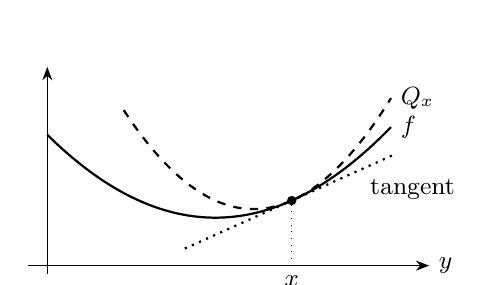
\begin{tikzpicture}[x=0.97cm,y=0.87cm,>=Stealth,font=\small]
  \draw[->] (-2.45,0)--(2.8,0) node[right] {$y$};
  \draw[->] (-2.2,-0.12)--(-2.2,2.9);
  % f(y)=0.25*y^2+0.7, anchor x=1, and a valid L=1 upper model.
  \draw[thick,domain=-2.2:2.3,samples=90]
    plot (\x,{0.25*(\x)^2+0.7});
  \draw[dashed,thick,domain=-1.2:2.3,samples=90]
    plot (\x,{0.95+0.5*(\x-1)+0.5*(\x-1)^2});
  \draw[dotted,thick] (-0.4,0.25)--(2.35,1.625);
  \fill (1,0.95) circle(1.7pt);
  \draw[dotted] (1,0)--(1,0.95);
  \node[below] at (1,0) {$x$};
  \node[right] at (2.3,2.445) {$Q_x$};
  \node[right] at (2.3,2.0225) {$f$};
  \node[below right] at (1.9,1.4) {tangent};
\end{tikzpicture}
\end{center}

Differentiate the quadratic model with respect to $y$:
\[
  Q_x'(y)=f'(x)+L(y-x).
\]
Setting this equal to zero gives its minimizer
\[
  y=\hide{x-\frac{f'(x)}{L}}.
\]
Thus gradient descent with $\eta=1/L$ minimizes a valid quadratic upper
bound at every iteration.

\begin{lemma}[One-step progress]\label{lem:descent}
For any $L$-smooth $f$, the point $x^+=x-f'(x)/L$ satisfies
\[
  \boxed{f(x^+)\leq f(x)-\frac{(f'(x))^2}{2L}.}
\]
\end{lemma}
\begin{proof}
Substitute $y=x-f'(x)/L$ into Lemma~\ref{lem:smooth}:
\[
 f(x^+)\leq f(x)-\frac{(f'(x))^2}{L}
              +\frac{L}{2}\frac{(f'(x))^2}{L^2}
          =f(x)-\frac{(f'(x))^2}{2L}.
\]
\end{proof}

% ======================== PAGE 12 ========================
\newpage
\section{The Algorithm and Its Two Possible Guarantees}

\begin{algorithm}[H]
\caption{Gradient-Descent$(f,x_0,L,T)$}\label{alg:gd}
\begin{algorithmic}[1]
  \Require Derivative access to an $L$-smooth function $f:\R\to\R$;
     $L>0$; initial point $x_0$; integer $T\geq1$
  \State $g_{\mathrm{best}}\gets+\infty$
  \For{$t=0,1,\ldots,T-1$}
    \State $g_t\gets f'(x_t)$
    \If{$|g_t|<g_{\mathrm{best}}$}
      \State $\widehat x\gets x_t$; $g_{\mathrm{best}}\gets |g_t|$
    \EndIf
    \State $x_{t+1}\gets x_t-g_t/L$
  \EndFor
  \State \Return $x_T$ and $\widehat x$
\end{algorithmic}
\end{algorithm}

\textbf{Which output?} We use $\widehat x$ for a small-derivative guarantee,
and $x_T$ for the convex objective-value guarantee. There is no need to
store all previous iterates: retaining the current point and the best
observed derivative magnitude is enough.

\textbf{Runtime.} The algorithm makes \hide{$T$} derivative queries.
If one derivative costs $C_{\mathrm{grad}}$ time, the total time is
\hide{$O(T(C_{\mathrm{grad}}+1))$} in the real-arithmetic model.

\begin{definition}
A point $x$ is an \textbf{$\eps$-critical point} if $|f'(x)|\leq\eps$.
A point $x$ is an \textbf{$\eps$-approximate minimizer} if
$f(x)-f(\xstar)\leq\eps$.
\end{definition}

These are \textbf{different guarantees}. Smoothness alone will let us find
an approximate critical point. Convexity and a distance bound will connect
criticality to global optimality.

\QU Let $f(x)=\cos x$. Gradient descent starts at $x_0=0$.
What happens, and is the output a local minimum?
\end{Qu}
\begin{answer}
Since $f'(0)=-\sin0=0$, every iterate remains at $0$.
But $f(0)=1$ is a global maximum, while $f(\pi)=-1$.
The function is $1$-smooth. Thus even an exactly critical point need not
be a local minimum of a smooth, nonconvex function.
\end{answer}
\vs{0.2in}

\textbf{Scope reminder.} We are minimizing over $\R$. At the boundary of a
constrained feasible set, an optimum need not have derivative zero.

% ======================== PAGE 13 ========================
\newpage
\section{Analysis I: Finding an Approximate Critical Point}

\begin{theorem}[Smooth, possibly nonconvex objective]\label{thm:critical}
Let $f:\R\to\R$ be $L$-smooth, with a minimizer $\xstar$, and suppose $\Delta\geq0$ satisfies
\[
  f(x_0)-f(\xstar)\leq\Delta.
\]
After $T\geq1$ iterations of Algorithm~\ref{alg:gd},
\[
  \boxed{\min_{0\leq t<T}|f'(x_t)|
          \leq\sqrt{\frac{2L\Delta}{T}}.}
\]
In particular, $T\geq 2L\Delta/\eps^2$ suffices for the returned
$\widehat x$ to be an $\eps$-critical point.
\end{theorem}

\textbf{Proof idea.} A large derivative forces a substantial decrease in
$f$. But the total decrease cannot exceed the initial gap $\Delta$.

\begin{proof}
By Lemma~\ref{lem:descent}, for every $0\leq t<T$,
\[
  \frac{(f'(x_t))^2}{2L}\leq f(x_t)-f(x_{t+1}).
\]
Sum over the $T$ iterations. The right-hand side telescopes:
\begin{align*}
  \frac{1}{2L}\sum_{t=0}^{T-1}(f'(x_t))^2
  &\leq f(x_0)-f(x_T)\\
  &\leq f(x_0)-f(\xstar)\leq\Delta.
\end{align*}
The smallest squared derivative is at most their average, so
\[
  \min_{0\leq t<T}(f'(x_t))^2
   \leq\frac1T\sum_{t=0}^{T-1}(f'(x_t))^2
   \leq\hide{\frac{2L\Delta}{T}}.
\]
Taking square roots proves the result.
\end{proof}

\QU Holding $L$ and $\Delta$ fixed, how does the sufficient iteration count
change if the desired derivative tolerance decreases from $\eps$ to
$\eps/2$?
\end{Qu}
\begin{answer}
It increases by a factor of $4$, since the bound is proportional to
$1/\eps^2$. Notice that no part of the proof used convexity.
\end{answer}

% ======================== PAGE 14 ========================
\newpage
\section{Analysis II: Adding Convexity}

For a convex objective, Lemma~\ref{lem:convexity} gives
\begin{align*}
 f(x)-f(\xstar)
 &\leq f'(x)(x-\xstar)\\
 &\leq |f'(x)|\,|x-\xstar|.
\end{align*}
A small derivative therefore gives a small objective gap \emph{provided}
we also control the distance to a minimizer.

\begin{lemma}[Distance never increases]\label{lem:distance}
Let $f:\R\to\R$ be convex and $L$-smooth, with minimizer $\xstar$.
For $x^+=x-f'(x)/L$,
\[
  |x^+-\xstar|\leq |x-\xstar|.
\]
Consequently, if $|x_0-\xstar|\leq R$, then $|x_t-\xstar|\leq R$
for every gradient-descent iterate.
\end{lemma}

\begin{proof}
Write $g=f'(x)$. Expanding the squared distance gives
\[
 (x^+-\xstar)^2
  =(x-\xstar)^2-\frac{2}{L}g(x-\xstar)+\frac{g^2}{L^2}.
\]
We need $g(x-\xstar)\geq g^2/(2L)$. To prove this, chain together
three facts:
\begin{align*}
  g(x-\xstar)
  &\geq f(x)-f(\xstar) &&\text{by convexity}\\
  &\geq f(x)-f(x^+) &&\text{by optimality of }\xstar\\
  &\geq \frac{g^2}{2L} &&\text{by one-step progress}.
\end{align*}
Substituting yields
\[
 (x^+-\xstar)^2
 \leq(x-\xstar)^2
   -\frac{2}{L}\frac{g^2}{2L}+\frac{g^2}{L^2}
 =(x-\xstar)^2.
\]
Both distances are nonnegative, so taking square roots proves the
one-step claim. Apply it repeatedly to obtain the statement for every $t$.
\end{proof}

\textbf{What to remember:} Smoothness controls how much a step can change
$f$; convexity supplies the inequality that also controls the distance.

% ======================== PAGE 15 ========================
\newpage
\subsection{A First Global Convergence Guarantee}

\begin{theorem}[Introductory convex guarantee]\label{thm:global}
Suppose $f:\R\to\R$ is convex and $L$-smooth, attains its minimum at
$\xstar$, and $|x_0-\xstar|\leq R$, where $R>0$. For every $T\geq1$,
Algorithm~\ref{alg:gd} satisfies
\[
  \boxed{f(x_T)-f(\xstar)\leq\frac{LR^2}{\sqrt T}.}
\]
Hence $T\geq L^2R^4/\eps^2$ suffices for an $\eps$-approximate minimizer.
\end{theorem}

\textbf{Proof idea.} Bound the initial objective gap, find a small
derivative, and use convexity together with the distance invariant.

\begin{proof}
\textbf{Step 1: Bound the initial gap.}
Since $\xstar$ is an unconstrained minimizer of a differentiable function,
$f'(\xstar)=0$. Center Lemma~\ref{lem:smooth} at $\xstar$:
\[
  f(x_0)-f(\xstar)
  \leq \frac L2(x_0-\xstar)^2
  \leq\frac{LR^2}{2}.
\]
Thus we may use $\Delta=LR^2/2$ in Theorem~\ref{thm:critical}.

\textbf{Step 2: Find an iterate with a small derivative.}
For some $0\leq t<T$,
\[
  |f'(x_t)|\leq\sqrt{\frac{2L\Delta}{T}}
          =\frac{LR}{\sqrt T}.
\]

\textbf{Step 3: Convert criticality to global optimality.}
Convexity and Lemma~\ref{lem:distance} imply
\[
  f(x_t)-f(\xstar)
  \leq |f'(x_t)|\,|x_t-\xstar|
  \leq \frac{LR}{\sqrt T}\,R=\frac{LR^2}{\sqrt T}.
\]
Finally, Lemma~\ref{lem:descent} says the objective values never increase.
Since $t<T$, we have $f(x_T)\leq f(x_t)$, which proves the claim for the
\emph{last} iterate.
\end{proof}

\textbf{Equivalent accuracy calculation.} To make the objective gap at
most $\eps$, it suffices to find a derivative of magnitude $\eps/R$:
\[
  \frac{2L(LR^2/2)}{(\eps/R)^2}
  =\hide{\frac{L^2R^4}{\eps^2}}\quad\text{iterations suffice.}
\]

% ======================== PAGE 16 ========================
\newpage
\section{The Higher-Dimensional Viewpoint}

Now let $x=(x_1,\ldots,x_d)\in\R^d$. A set $\X\subseteq\R^d$ is
\textbf{convex} if it contains the entire line segment between every pair
of its points:
\[
  x,y\in\X,\ \lambda\in[0,1]
  \quad\Longrightarrow\quad (1-\lambda)x+\lambda y\in\X.
\]
A function $f:\X\to\R$ is convex if $\X$ is convex and
\[
 f((1-\lambda)x+\lambda y)
 \leq (1-\lambda)f(x)+\lambda f(y).
\]
Minimizing a convex function over a convex set is a
\hide{\textbf{convex optimization problem}}. Our gradient-descent analysis
concerns the unconstrained case $\X=\R^d$.

\paragraph{Replace the derivative with a gradient.}
For differentiable $f:\R^d\to\R$, the gradient is
\[
 \nabla f(x)=\begin{pmatrix}
  \partial f(x)/\partial x_1\\
  \vdots\\
  \partial f(x)/\partial x_d
 \end{pmatrix}.
\]
Write $\langle u,v\rangle=\sum_i u_iv_i$ and
$\|u\|_2=\sqrt{\sum_i u_i^2}$.
Euclidean $L$-smoothness means
\[
  \|\nabla f(x)-\nabla f(y)\|_2\leq L\|x-y\|_2.
\]
The update becomes
\[
  \boxed{x_{t+1}=x_t-\frac1L\nabla f(x_t).}
\]

\begin{example}\textbf{A Two-Dimensional Step}
Let $f(u,v)=u^2+4v^2$. Verify that $L=8$ is valid, and take one gradient
descent step from $(2,1)$ with $\eta=1/8$.
\end{example}
\begin{answer}
The gradient is $(2u,8v)$, and
$\|(2a,8b)\|_2^2=4a^2+64b^2\leq64(a^2+b^2)$.
At $(2,1)$, the gradient is $(4,8)$, so the next point is
$(2,1)-(4,8)/8=(3/2,0)$. A single step size need not solve both
coordinates in one step.
\end{answer}

% ======================== PAGE 17 ========================
\newpage
\subsection{The Same Analysis, With Inner Products and Norms}

The two central inequalities generalize to
\begin{align*}
 f(y)&\geq f(x)+\langle\nabla f(x),y-x\rangle
          &&\text{(convexity)},\\
 f(y)&\leq f(x)+\langle\nabla f(x),y-x\rangle
                  +\frac L2\|y-x\|_2^2
          &&\text{(smoothness)}.
\end{align*}
In particular, the same substitution into the upper bound gives
\[
 f\left(x-\frac1L\nabla f(x)\right)
 \leq f(x)-\frac{\|\nabla f(x)\|_2^2}{2L}.
\]
The telescoping proof therefore gives
\[
  \min_{0\leq t<T}\|\nabla f(x_t)\|_2
  \leq\sqrt{\frac{2L\Delta}{T}}.
\]
For the convex guarantee, replace squared scalar distances by squared
Euclidean distances in Lemma~\ref{lem:distance}, and use Cauchy--Schwarz:
\[
  f(x)-f(\xstar)
  \leq\langle\nabla f(x),x-\xstar\rangle
  \leq\|\nabla f(x)\|_2\,\|x-\xstar\|_2.
\]
Thus the introductory bound in Theorem~\ref{thm:global} also holds when
$\|x_0-\xstar\|_2\leq R$.

\textbf{Iterations are not the same as runtime.} There is no explicit $d$
in these iteration bounds. However, $L$, $R$, and the cost of a gradient
can depend on $d$. Each vector update also takes $O(d)$ arithmetic
operations, so $T$ iterations cost
\[
  O\bigl(T(C_{\mathrm{grad}}+d)\bigr).
\]

\QU Which statement is justified by today's analysis?
\begin{enumerate}
  \aitem A small gradient always means a nearby minimizer.
  \bitem Smoothness alone guarantees a global minimum.
  \citem A constant number of scalar arithmetic operations always suffices
  for one iteration, regardless of $d$.
  \ditem Smoothness guarantees progress proportional to the squared
  gradient norm; convexity can turn local information into a global bound.
\end{enumerate}
\end{Qu}
% Answer: D.
\begin{answer}
\textbf{Answer: D.} A confuses derivative size with distance to a
minimizer; B assumes smoothness implies global optimality; C ignores the
cost of processing $d$ coordinates.
\end{answer}

% ======================== PAGE 18 ========================
\newpage
\section{Summary and Beyond Today's Analysis}

\paragraph{The algorithm.}
Start from $x_0$ and repeatedly use the local slope to improve the current
guess. In one dimension,
\[
  x_{t+1}=x_t-\frac1L f'(x_t).
\]
In $\R^d$, replace $f'(x_t)$ with $\nabla f(x_t)$.

\paragraph{The role of each assumption.}
\textbf{Smoothness} gives a quadratic upper bound and a safe step size.
\textbf{Convexity} gives a linear lower bound and rules out nonglobal local
minima. A bound on the initial gap or distance turns these structural
statements into an iteration count.

\paragraph{The guarantees proved in this lecture.}
For a smooth objective with initial value gap at most $\Delta$,
\[
  T\geq\frac{2L\Delta}{\eps^2}
  \quad\Longrightarrow\quad
  \text{an $\eps$-critical point among the queried iterates}.
\]
For a smooth convex objective with initial distance at most $R$,
\[
  T\geq\frac{L^2R^4}{\eps^2}
  \quad\Longrightarrow\quad
  f(x_T)-f(\xstar)\leq\eps.
\]
Take the ceiling of the displayed iteration bound, and at least one
iteration. These results assume an attained optimum and exact gradients.

\paragraph{Stronger results: stated, not proved here.}
The supplied notes, Section 2.4, point out that a sharper analysis of the
\emph{same} gradient-descent algorithm gives an $\eps$-approximate minimizer
in $O(LR^2/\eps)$ iterations. The $1/\eps^2$ dependence above is a limitation
of our introductory proof, not the best bound for gradient descent.

The notes also describe \textbf{acceleration}: an appropriately modified
algorithm using momentum attains $O(\sqrt{LR^2/\eps})$ iterations for smooth
convex minimization. Arbitrarily adding momentum does not inherit this
guarantee; the method and its analysis are beyond today's lecture.

\paragraph{Sources.}
Kevin Tian, \emph{CS331, Part VI: Continuous Algorithms}, Sections 1--2
(especially Lemmas 1--5) and Section 5.1; and \emph{CS331, Fall 2025,
Lecture 15 (10/20)}. These sources supply the theory and lecture sequence.
Exercises and questions were written for this adaptation.

\end{document}
'
%
% Source scope: Part6_main.pdf, Sections 1--2 (main lecture), and
% Section 5.1 (definition of a convex set in the final extension).
% The companion 10-20.pdf supplies the one-dimensional-first progression.
% New numerical examples and questions are practice exercises, not quotations.

\documentclass[11pt,letterpaper]{article}
\usepackage[lmargin=1in,rmargin=1.75in,bmargin=1in,tmargin=1in]{geometry}
\usepackage[T1]{fontenc}
\usepackage{lmodern}
\usepackage{amsmath,amssymb,amsthm}
\usepackage{graphicx}
\usepackage{setspace}
\usepackage{enumitem}
\usepackage{algorithm}
\usepackage{algpseudocode}
\usepackage{float}
\usepackage{tikz}
\usepackage{environ}
\usepackage{fancyhdr}
\usepackage{microtype}
\usepackage[hidelinks]{hyperref}
\usetikzlibrary{arrows.meta}

% ---------------- Editable course information ----------------
\newcommand{\CourseName}{CSCE 411: Design and Analysis of Algorithms}
\newcommand{\LectureDate}{} % Fill in the actual lecture date here.
\newcommand{\LectureNumber}{} % Optional, e.g., 15: (include the colon).

% ---------------- Standalone course-style definitions ----------------
\newif\ifstudentversion
\studentversionfalse
\ifdefined\studenthandout\studentversiontrue\fi
\newcommand{\vs}[1]{\vspace{#1}}
\newcommand{\hide}[1]{%
  \ifstudentversion
    \ifmmode\phantom{#1}\else\underline{\phantom{#1}}\fi
  \else #1\fi}
\newcommand{\lecture}[2]{%
  \noindent\textbf{\CourseName}\hfill #2\par
  \vspace{5pt}\hrule\vspace{10pt}
  {\centering\Large\bfseries #1\par}
  \vspace{10pt}\hrule\vspace{9pt}}
\theoremstyle{definition}
\newtheorem{definition}{Definition}
\newtheorem{example}{Example}
\theoremstyle{plain}
\newtheorem{lemma}{Lemma}
\newtheorem{theorem}{Theorem}
\newtheorem{fact}{Fact}
\newcounter{question}
\newenvironment{Qu}{%
  \par\medskip\refstepcounter{question}
  \noindent\textbf{Question \thequestion.}\ }{\par\medskip}
\newcommand{\QU}{\begin{Qu}}
\newcommand{\aitem}{\item[\textbf{(A)}]}
\newcommand{\bitem}{\item[\textbf{(B)}]}
\newcommand{\citem}{\item[\textbf{(C)}]}
\newcommand{\ditem}{\item[\textbf{(D)}]}
\newcommand{\eitem}{\item[\textbf{(E)}]}
\newsavebox{\answerbox}
% Answers occupy the same space in both versions; in the student version
% this space is left blank for the in-class calculation or discussion.
\NewEnviron{answer}{%
  \par\begingroup
  \setbox\answerbox=\vbox{\hsize=\linewidth\parindent=0pt\BODY\par}%
  \noindent\ifstudentversion\phantom{\usebox{\answerbox}}%
  \else\usebox{\answerbox}\fi\par\endgroup}
\newenvironment{problemframe}{%
  \par\smallskip\noindent
  \begin{lrbox}{\answerbox}
  \begin{minipage}{\dimexpr\linewidth-2\fboxsep-2\fboxrule\relax}}%
  {\end{minipage}\end{lrbox}\fbox{\usebox{\answerbox}}\par\smallskip}
\newcommand{\R}{\mathbb R}
\newcommand{\X}{\mathcal X}
\newcommand{\eps}{\varepsilon}
\newcommand{\xstar}{x^\star}
\DeclareMathOperator*{\argmin}{arg\,min}
\setlength{\parindent}{0pt}
\setlength{\parskip}{5pt}
\setlength{\headheight}{14pt}
\setlist[itemize]{topsep=3pt,itemsep=2pt,parsep=0pt}
\setlist[enumerate]{topsep=3pt,itemsep=2pt,parsep=0pt,leftmargin=2.1em}
\pagestyle{fancy}
\fancyhf{}
\fancyhead[L]{\small Convex Optimization and Gradient Descent}
\fancyhead[R]{\small CSCE 411}
\fancyfoot[C]{\thepage}
\renewcommand{\headrulewidth}{0.3pt}
\renewcommand{\footrulewidth}{0pt}
\raggedbottom
\hypersetup{pdftitle={Introduction to Convex Optimization and Gradient Descent},
  pdfauthor={CSCE 411 Lecture Notes},pdfsubject={Design and Analysis of Algorithms}}

\begin{document}
\onehalfspacing
\thispagestyle{plain}

% ======================== PAGE 1 ========================
\lecture{\LectureNumber\ Introduction to Convex Optimization\\and Gradient Descent}{\LectureDate}

\paragraph{Reading.}
Kevin Tian, \emph{Part VI: Continuous Algorithms}, Sections 1--2;
and the accompanying October 20 lecture notes. The last section briefly
introduces the higher-dimensional viewpoint from Section 5.1.

\section{Motivation: From Discrete to Continuous Optimization}

Many problems we have studied ask us to choose the best object from a set of
possible objects. We can write this common form as
\[
  \min_{x\in\X} f(x)
  \qquad\text{or}\qquad
  \max_{x\in\X} f(x).
\]
The variable $x$ is the \hide{\textbf{decision variable}}, the set $\X$ is the
\hide{\textbf{feasible set}}, and $f$ is the \hide{\textbf{objective function}}.

\begin{center}
\renewcommand{\arraystretch}{1.25}
\begin{tabular}{lll}
\textbf{Problem} & \textbf{Feasible objects} & \textbf{Objective}\\\hline
Interval scheduling & Nonoverlapping subsets & Maximize subset size\\
Minimum spanning tree & Spanning trees & Minimize total weight\\
Shortest path & $s$--$t$ paths & Minimize total weight
\end{tabular}
\end{center}

In these examples, the choices are discrete. Today, the decision variable
can instead be a real number or a vector of real numbers: $x\in\X\subseteq\R^d$.
There may be infinitely many feasible choices!

\begin{example}\textbf{Approximate Continuous Minimization}
\begin{problemframe}
\textbf{Input:} A function $f:\X\to\R$, a nonempty feasible set
$\X\subseteq\R^d$, and an accuracy parameter $\eps>0$.

\textbf{Output:} A point $\widehat x\in\X$ satisfying
\[
  f(\widehat x)\leq \hide{f(\xstar)+\eps},
  \qquad \xstar\in\argmin_{x\in\X} f(x).
\]
Here we assume that a minimizer $\xstar$ exists.
\end{problemframe}
\end{example}

Our accuracy target concerns the \emph{objective value}, not necessarily the
location of the output. An additive error of $\eps$ need not imply
$|\widehat x-\xstar|\leq\eps$.

% ======================== PAGE 2 ========================
\newpage
\subsection{A Familiar Example: Maximum Flow}

A maximum-flow problem already has a continuous formulation. Let
$G=(V,E)$ be a directed graph, with source $s$, sink $t$, and capacities
$c_e\geq0$. For this formulation, assume no edges enter $s$ or leave $t$.
Let $x_e$ denote the flow on edge $e$, so the decision variable is
$x\in\R^{|E|}$.

We want to maximize
\[
  f(x)=\sum_{e=(s,v)\in E}x_e
\]
subject to the constraints
\begin{align*}
  0\leq x_e&\leq c_e &&\text{for every }e\in E,\\
  \sum_{e=(u,v)\in E}x_e&=
  \sum_{e=(v,w)\in E}x_e &&\text{for every }v\in V\setminus\{s,t\}.
\end{align*}
The first constraints enforce \hide{capacity bounds}; the second enforce
\hide{flow conservation}. The feasible set $\X$ contains every flow satisfying
these constraints.

\QU Suppose there is a nonzero feasible flow $x$. Why are there infinitely
many feasible flows, even though the graph is finite?
\end{Qu}
\begin{answer}
For every $\lambda\in[0,1]$, the scaled flow $\lambda x$ is feasible:
capacity inequalities and conservation are preserved. Because $x\neq0$,
different values of $\lambda$ give different flows.
\end{answer}
\vs{0.25in}

\subsection{Another Motivation: Fitting a Model to Data}

Suppose $x\in\R^d$ records the parameters of a prediction rule. We can use a
\textbf{loss function} $f(x)$ to measure its errors on a collection of
training examples, and choose the parameters by minimizing $f(x)$.

There are infinitely many parameter choices, so enumerating all models is
not an option. Instead, we will repeatedly improve a current guess using
local information about the objective.

\textbf{Important distinction.} The loss of a complicated model need not be
convex. Our analysis will separate what smoothness alone guarantees from
what additionally requires convexity.

% ======================== PAGE 3 ========================
\newpage
\section{What Information Can an Algorithm Use?}

In the \hide{\textbf{oracle model}}, we ask for information about $f$ at
points of our choice. A \textbf{value query} returns $f(x)$; a
\textbf{derivative query} returns $f'(x)$ in one dimension.
We count queries separately from the cost of computing them.
For the gradient-descent theorems, we assume exact derivative queries and
exact real arithmetic.

Derivative queries are natural because a derivative describes how the
function changes nearby. Value queries can also \emph{approximate} a
derivative through
\[
  f'(x)\approx\frac{f(x+\delta)-f(x)}{\delta},
  \qquad \delta>0.
\]
We will make the approximation error precise after defining smoothness.

\subsection{Without Structure, Queries May Tell Us Nothing}

For an unknown point $z\in[0,1]$, consider
\[
  f_z(x)=
  \begin{cases}
    0,&x=z,\\
    1,&x\neq z.
  \end{cases}
\]
Even finding $\widehat x$ with $f_z(\widehat x)\leq\min f_z+0.99$ requires
finding \hide{the exact point $z$}.

\textbf{Why finitely many queries cannot guarantee success.}
Consider a deterministic algorithm and answer every query with $1$.
After its finite query sequence and output $\widehat x$, choose $z$ outside
all queried points and outside $\{\widehat x\}$. Every answer is consistent
with $f_z$, but the output has value $1$ while the minimum is $0$.

\textbf{Takeaway:} A bounded domain and bounded function values are not
enough. We need assumptions under which queries provide useful information.

\paragraph{A contrasting example: unimodality.}
If $f$ is strictly decreasing up to a minimizer $c$ and strictly increasing
afterward, compare its values at
\[
  u=\ell+\frac{r-\ell}{3},\qquad
  v=\ell+\frac{2(r-\ell)}{3}
\]
in a known interval $[\ell,r]$ containing $c$. If $f(u)<f(v)$, discard
$(v,r]$; if $f(u)>f(v)$, discard $[\ell,u)$; if they are equal, retain $[u,v]$.
This is \hide{\textbf{ternary search}}: local queries now reveal which
part of the interval can contain the minimizer.

% ======================== PAGE 4 ========================
\newpage
\section{Convexity: Structure That Helps Optimization}

We first work in \textbf{one dimension}. Unless otherwise specified,
$f:\R\to\R$, and we minimize over all of $\R$.

\begin{definition}
A function $f:\R\to\R$ is \hide{\textbf{convex}} if, for every $x,y\in\R$
and every $\lambda\in[0,1]$,
\[
  \boxed{f((1-\lambda)x+\lambda y)
  \leq (1-\lambda)f(x)+\lambda f(y).}
\]
\end{definition}

The point $(1-\lambda)x+\lambda y$ is a weighted average of $x$ and $y$.
The right-hand side is the height of the line segment joining
$(x,f(x))$ and $(y,f(y))$. A convex function lies \hide{at or below}
every such segment.

\begin{center}
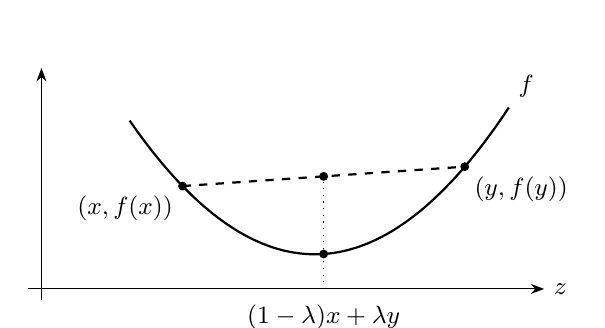
\begin{tikzpicture}[x=1.12cm,y=1.1cm,>=Stealth,font=\small]
  \draw[->] (-1.25,0)--(4.6,0) node[right] {$z$};
  \draw[->] (-1.1,-0.13)--(-1.1,2.55);
  \draw[thick,domain=-0.1:4.2,samples=90]
    plot (\x,{0.35*(\x-2)^2+0.4});
  \draw[thick,dashed] (0.5,1.1875)--(3.7,1.4115);
  \fill (0.5,1.1875) circle(1.6pt) node[below left] {$(x,f(x))$};
  \fill (3.7,1.4115) circle(1.6pt) node[below right] {$(y,f(y))$};
  \draw[dotted] (2.1,0)--(2.1,1.2995);
  \fill (2.1,0.4035) circle(1.6pt);
  \fill (2.1,1.2995) circle(1.6pt);
  \node[below,align=center] at (2.1,-0.07) {$(1-\lambda)x+\lambda y$};
  \node[above right] at (4.2,2.094) {$f$};
\end{tikzpicture}
\end{center}

\QU Which of the following functions are convex on $\R$?
\[
  f_1(x)=x^2,\quad f_2(x)=|x|,\quad
  f_3(x)=3x+1,\quad f_4(x)=-x^2.
\]
\begin{enumerate}
  \aitem Only $f_1$.
  \bitem Only $f_1$ and $f_2$.
  \citem $f_1$, $f_2$, and $f_3$.
  \ditem All four functions.
\end{enumerate}
\end{Qu}
% Answer: C.
\begin{answer}
\textbf{Answer: C.} Convex functions need not be differentiable: $|x|$ has a
corner at $0$. Linear functions satisfy the convexity inequality with
equality. For $-x^2$, take $x=-1$, $y=1$, and $\lambda=1/2$:
the proposed inequality would be $0\leq-1$.
\end{answer}

% ======================== PAGE 5 ========================
\newpage
\subsection{A Second View: Convex Functions Lie Above Their Tangents}

If $f$ is differentiable, its linear, or \textbf{Euler}, approximation at
$x$ is
\[
  f(x)+f'(x)(y-x).
\]
For a general function, this is only a local approximation. For a convex
function, it gives a \hide{global lower bound}.

\begin{lemma}[First-order inequality]\label{lem:convexity}
If $f:\R\to\R$ is differentiable and convex, then, for all $x,y\in\R$,
\[
  \boxed{f(y)\geq f(x)+f'(x)(y-x).}
\]
\end{lemma}

\begin{proof}
For $0<\lambda\leq1$, convexity gives
\[
  f(x+\lambda(y-x))\leq(1-\lambda)f(x)+\lambda f(y).
\]
Rearrange, dividing by the positive number $\lambda$:
\[
  f(y)\geq f(x)+\frac{f(x+\lambda(y-x))-f(x)}{\lambda}.
\]
Let $\lambda\to0^+$. The quotient tends to
\hide{$f'(x)(y-x)$}, which proves the inequality.
\end{proof}

\vs{0.2in}
\textbf{Two compatible pictures of convexity:}
\[
  \text{below every \hide{chord}}
  \qquad\text{and}\qquad
  \text{above every \hide{tangent}}.
\]

\QU Suppose $f$ is differentiable and convex, and $f'(x)=0$.
What can we conclude?
\begin{enumerate}
  \aitem $x$ is necessarily the unique minimizer.
  \bitem $x$ is a global minimizer, but need not be unique.
  \citem $x$ could be a strict local maximum.
  \ditem Nothing about optimality.
\end{enumerate}
\end{Qu}
% Answer: B.
\begin{answer}
\textbf{Answer: B.} For every $y$, the first-order inequality yields
$f(y)\geq f(x)+0\cdot(y-x)=f(x)$. A constant function shows that the
minimizer need not be unique.
\end{answer}

% ======================== PAGE 6 ========================
\newpage
\subsection{Why Local Information Is Useful}

\begin{lemma}[Local minima are global minima]
For a convex function, every local minimum is a global minimum.
\end{lemma}
\begin{proof}
Suppose $x$ is a local minimum but $f(y)<f(x)$ for some $y$.
For sufficiently small $\lambda>0$, the point
$z=(1-\lambda)x+\lambda y$ lies in the neighborhood where $x$ is a minimum.
But
\[
  f(z)\leq(1-\lambda)f(x)+\lambda f(y)<f(x),
\]
which is a contradiction. This argument does not require differentiability.
\end{proof}

\paragraph{The derivative points toward improvement.}
Let $\xstar$ be a minimizer. If $f'(x)>0$, then, for every $y>x$,
\[
  f(y)\geq f(x)+f'(x)(y-x)>f(x).
\]
Thus no minimizer lies to the \hide{right} of $x$. Similarly, if
$f'(x)<0$, no minimizer lies to the \hide{left} of $x$.
Given an interval containing a minimizer, these tests permit binary search.
If $f'(x)=0$, we have already found a global minimizer.

\begin{fact}[Calculus test]
For twice-differentiable $f:\R\to\R$, convexity is equivalent to
$f''(x)\geq0$ for all $x$. Equivalently, $f'$ is nondecreasing.
\end{fact}

\section{Gradient Descent: Move Instead of Discard}

A one-dimensional interval has a natural left and right. In high dimensions,
there is no direct analogue of this interval-based binary search.
An alternative is to move our current point using its derivative:
\[
  \boxed{x_{t+1}=x_t-\eta f'(x_t).}
\]
This is \hide{\textbf{gradient descent}}. The parameter $\eta>0$ is the
\hide{\textbf{step size}}.

\textbf{The design question:} How should we choose $\eta$? Too small may
mean very slow progress; too large may overshoot the minimizer and even
increase the objective. Moving in a descent direction is not, by itself,
a guarantee that an arbitrary-length step decreases $f$.

% ======================== PAGE 7 ========================
\newpage
\section{Smoothness: How Far Can We Safely Move?}

We need a condition that prevents the derivative from changing too quickly.
First, recall a related condition on function values.

\begin{definition}
Let $G\geq0$ and $L>0$. A function $f:\R\to\R$ is
\textbf{$G$-Lipschitz} if, for all $x,y\in\R$,
\[
  |f(x)-f(y)|\leq G|x-y|.
\]
A differentiable function $f:\R\to\R$ is \textbf{$L$-smooth} if, for all
$x,y\in\R$,
\[
  \boxed{|f'(x)-f'(y)|\leq L|x-y|.}
\]
\end{definition}

Lipschitzness of $f$ controls its \hide{values}; smoothness controls its
\hide{derivative}. We use $G$ and $L$ to distinguish these two bounds.

\textbf{Useful calculus tests.} On $\R$, for differentiable $f$,
$|f'|\leq G$ everywhere is equivalent to $G$-Lipschitzness.
For twice-differentiable $f$, $|f''|\leq L$ everywhere is equivalent to
$L$-smoothness.

\QU Classify each function on \emph{all of $\R$}.
\begin{center}
\renewcommand{\arraystretch}{1.35}
\begin{tabular}{lccc}
 & \textbf{Convex?} & \textbf{Lipschitz?} & \textbf{Smooth?}\\\hline
$x^2$ & \hide{Yes} & \hide{No} & \hide{Yes, $L=2$}\\
$|x|$ & \hide{Yes} & \hide{Yes, $G=1$} & \hide{No}\\
$\cos x$ & \hide{No} & \hide{Yes, $G=1$} & \hide{Yes, $L=1$}
\end{tabular}
\end{center}
\end{Qu}

\paragraph{What about simulating derivative queries?}
For $L$-smooth $f$ and $\delta>0$, the fundamental theorem of calculus gives
\begin{align*}
 \left|\frac{f(x+\delta)-f(x)}{\delta}-f'(x)\right|
 &\leq\frac{1}{\delta}\int_0^\delta|f'(x+s)-f'(x)|\,ds\\
 &\leq\frac{1}{\delta}\int_0^\delta Ls\,ds
 =\frac{L\delta}{2}.
\end{align*}
This is an \emph{approximation}, not an exact simulation. Our theorems use
exact derivative queries; finite-difference and floating-point errors are
not included in those guarantees.

% ======================== PAGE 8 ========================
\newpage
\section{Gradient Descent, Take 1: Quadratics}

The simplest smooth convex functions are quadratics. Let
\[
  q(x)=ax^2+bx+c,\qquad a>0.
\]
We can analyze gradient descent exactly in this case.

\paragraph{Where is the minimizer?}
Complete the square:
\begin{align*}
  q(x)
  &=a\left(x+\frac{b}{2a}\right)^2+c-\frac{b^2}{4a},\\[4pt]
  \xstar&=\hide{-\frac{b}{2a}}.
\end{align*}
The additive constant does not affect the location of the minimizer.
The error in the objective value is
\[
  q(x)-q(\xstar)=\hide{a(x-\xstar)^2}.
\]

\paragraph{What does the derivative tell us?}
\[
  q'(x)=2ax+b=\hide{2a(x-\xstar)}.
\]
Thus the derivative is exactly proportional to the signed distance from
the current point to the minimizer. Moreover,
\[
  |q'(x)-q'(y)|=2a|x-y|,
\]
so the tight smoothness constant is \hide{$L=2a$}.

\begin{example}\textbf{Complete the Square}
Let $q(x)=x^2-6x+10$. Find the minimizer, the minimum value, the derivative,
and a tight smoothness constant.
\end{example}
\begin{answer}
\begin{align*}
  q(x)&=(x-3)^2+1,&\xstar&=3,\\
  q(\xstar)&=1,&q'(x)&=2x-6,\qquad L=2.
\end{align*}
\end{answer}
\vs{0.4in}

\textbf{Next question:} Can we choose a step size that lands directly at
$\xstar$?

% ======================== PAGE 9 ========================
\newpage
\subsection{Choosing and Testing the Step Size}

For a quadratic with tight smoothness constant $L=2a$, a gradient step is
\[
  x_{t+1}=x_t-\eta L(x_t-\xstar).
\]
Subtracting $\xstar$ from both sides gives the exact recurrence
\[
  \boxed{x_{t+1}-\xstar=(1-\eta L)(x_t-\xstar).}
\]
With $\eta=\hide{1/L}$, the multiplier is zero: we reach the minimizer in
\hide{one step}. A larger valid upper bound on smoothness gives a smaller,
still safe step, but need not give one-step convergence.

\begin{example}\textbf{Trace the Iterates}
Use $q(x)=x^2-6x+10$, $x_0=0$, and $L=2$. Compute $x_1$ and $x_2$ for each
choice of $\eta$.
\begin{center}
\renewcommand{\arraystretch}{1.6}
\begin{tabular}{c|cc|l}
$\eta$ & $x_1$ & $x_2$ & \textbf{Behavior}\\\hline
$1/4$ & \hide{$3/2$} & \hide{$9/4$} & \hide{Approaches from one side}\\
$1/2$ & \hide{$3$} & \hide{$3$} & \hide{Reaches the minimizer}\\
$3/4$ & \hide{$9/2$} & \hide{$9/4$} & \hide{Alternates, but gets closer}\\
$1$ & \hide{$6$} & \hide{$0$} & \hide{Oscillates without progress}
\end{tabular}
\end{center}
\end{example}

\QU Does overshooting always imply that gradient descent diverges?
Use the recurrence to determine exactly when the distance decreases
for this quadratic.
\end{Qu}
\begin{answer}
No. The distance decreases at every nonoptimal iterate precisely when
\[
  |1-\eta L|<1\quad\Longleftrightarrow\quad 0<\eta<\frac{2}{L}.
\]
For $1/L<\eta<2/L$, the iterates cross the minimizer but get closer.
At $\eta=2/L$, a nonoptimal starting point oscillates. For $\eta>2/L$, its
distance grows. Thus $1/L$ is a convenient safe choice, not the only
convergent choice for a quadratic.
\end{answer}
\vs{0.15in}

\textbf{Progress with $\eta=1/L$:}
\[
  q(x)-q\left(x-\frac{q'(x)}{L}\right)
  =a(x-\xstar)^2=\hide{\frac{(q'(x))^2}{2L}}.
\]

% ======================== PAGE 10 ========================
\newpage
\section{Gradient Descent, Take 2: Smooth Functions}

A general smooth function is not a quadratic. The useful replacement is
that it has a \textbf{quadratic upper bound} centered at every point.

\begin{lemma}[Quadratic upper bound]\label{lem:smooth}
If $f:\R\to\R$ is $L$-smooth, then, for every $x,y\in\R$,
\[
  \boxed{f(y)\leq f(x)+f'(x)(y-x)+\frac L2(y-x)^2.}
\]
Convexity is \emph{not} required.
\end{lemma}

\textbf{Intuition.} A first-order approximation uses the tangent line.
Smoothness controls how far the derivative can move away from its initial
value, so the error accumulated along a step is at most quadratic in the
step length.

\begin{proof}
Write $h=y-x$. Parameterizing the segment from $x$ to $y$ by $x+sh$, where
$0\leq s\leq1$, gives
\begin{align*}
 f(y)-f(x)-f'(x)h
   &=\int_0^1\bigl(f'(x+sh)-f'(x)\bigr)h\,ds\\
   &\leq\int_0^1|f'(x+sh)-f'(x)|\,|h|\,ds\\
   &\leq\int_0^1 Ls|h|^2\,ds\\
   &=\hide{\frac L2 h^2}.
\end{align*}
The absolute values make the argument valid whether $y\geq x$ or $y<x$.
Substitute $h=y-x$ and rearrange.
\end{proof}

\vs{0.25in}
For a function that is \emph{both convex and $L$-smooth}, we now have
\begin{align*}
  f(x)+f'(x)(y-x)
  &\leq f(y)\\
  &\leq f(x)+f'(x)(y-x)+\frac L2(y-x)^2.
\end{align*}
Convexity supplies the \hide{linear lower bound}.\\
Smoothness supplies the \hide{quadratic upper bound}.\\
These two inequalities play different roles in the analysis.

% ======================== PAGE 11 ========================
\newpage
\subsection{Minimize the Upper Bound, Not the Unknown Function}

At the current point $x$, define the quadratic model
\[
  Q_x(y)=f(x)+f'(x)(y-x)+\frac L2(y-x)^2.
\]
We know $Q_x(x)=f(x)$ and $f(y)\leq Q_x(y)$ for all $y$.

\begin{center}
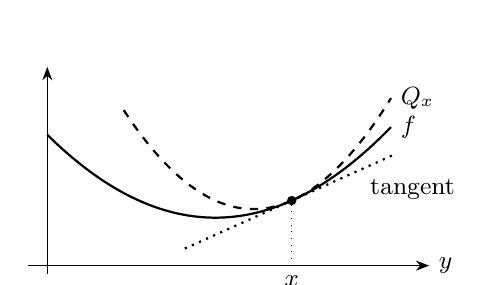
\begin{tikzpicture}[x=0.97cm,y=0.87cm,>=Stealth,font=\small]
  \draw[->] (-2.45,0)--(2.8,0) node[right] {$y$};
  \draw[->] (-2.2,-0.12)--(-2.2,2.9);
  % f(y)=0.25*y^2+0.7, anchor x=1, and a valid L=1 upper model.
  \draw[thick,domain=-2.2:2.3,samples=90]
    plot (\x,{0.25*(\x)^2+0.7});
  \draw[dashed,thick,domain=-1.2:2.3,samples=90]
    plot (\x,{0.95+0.5*(\x-1)+0.5*(\x-1)^2});
  \draw[dotted,thick] (-0.4,0.25)--(2.35,1.625);
  \fill (1,0.95) circle(1.7pt);
  \draw[dotted] (1,0)--(1,0.95);
  \node[below] at (1,0) {$x$};
  \node[right] at (2.3,2.445) {$Q_x$};
  \node[right] at (2.3,2.0225) {$f$};
  \node[below right] at (1.9,1.4) {tangent};
\end{tikzpicture}
\end{center}

Differentiate the quadratic model with respect to $y$:
\[
  Q_x'(y)=f'(x)+L(y-x).
\]
Setting this equal to zero gives its minimizer
\[
  y=\hide{x-\frac{f'(x)}{L}}.
\]
Thus gradient descent with $\eta=1/L$ minimizes a valid quadratic upper
bound at every iteration.

\begin{lemma}[One-step progress]\label{lem:descent}
For any $L$-smooth $f$, the point $x^+=x-f'(x)/L$ satisfies
\[
  \boxed{f(x^+)\leq f(x)-\frac{(f'(x))^2}{2L}.}
\]
\end{lemma}
\begin{proof}
Substitute $y=x-f'(x)/L$ into Lemma~\ref{lem:smooth}:
\[
 f(x^+)\leq f(x)-\frac{(f'(x))^2}{L}
              +\frac{L}{2}\frac{(f'(x))^2}{L^2}
          =f(x)-\frac{(f'(x))^2}{2L}.
\]
\end{proof}

% ======================== PAGE 12 ========================
\newpage
\section{The Algorithm and Its Two Possible Guarantees}

\begin{algorithm}[H]
\caption{Gradient-Descent$(f,x_0,L,T)$}\label{alg:gd}
\begin{algorithmic}[1]
  \Require Derivative access to an $L$-smooth function $f:\R\to\R$;
     $L>0$; initial point $x_0$; integer $T\geq1$
  \State $g_{\mathrm{best}}\gets+\infty$
  \For{$t=0,1,\ldots,T-1$}
    \State $g_t\gets f'(x_t)$
    \If{$|g_t|<g_{\mathrm{best}}$}
      \State $\widehat x\gets x_t$; $g_{\mathrm{best}}\gets |g_t|$
    \EndIf
    \State $x_{t+1}\gets x_t-g_t/L$
  \EndFor
  \State \Return $x_T$ and $\widehat x$
\end{algorithmic}
\end{algorithm}

\textbf{Which output?} We use $\widehat x$ for a small-derivative guarantee,
and $x_T$ for the convex objective-value guarantee. There is no need to
store all previous iterates: retaining the current point and the best
observed derivative magnitude is enough.

\textbf{Runtime.} The algorithm makes \hide{$T$} derivative queries.
If one derivative costs $C_{\mathrm{grad}}$ time, the total time is
\hide{$O(T(C_{\mathrm{grad}}+1))$} in the real-arithmetic model.

\begin{definition}
A point $x$ is an \textbf{$\eps$-critical point} if $|f'(x)|\leq\eps$.
A point $x$ is an \textbf{$\eps$-approximate minimizer} if
$f(x)-f(\xstar)\leq\eps$.
\end{definition}

These are \textbf{different guarantees}. Smoothness alone will let us find
an approximate critical point. Convexity and a distance bound will connect
criticality to global optimality.

\QU Let $f(x)=\cos x$. Gradient descent starts at $x_0=0$.
What happens, and is the output a local minimum?
\end{Qu}
\begin{answer}
Since $f'(0)=-\sin0=0$, every iterate remains at $0$.
But $f(0)=1$ is a global maximum, while $f(\pi)=-1$.
The function is $1$-smooth. Thus even an exactly critical point need not
be a local minimum of a smooth, nonconvex function.
\end{answer}
\vs{0.2in}

\textbf{Scope reminder.} We are minimizing over $\R$. At the boundary of a
constrained feasible set, an optimum need not have derivative zero.

% ======================== PAGE 13 ========================
\newpage
\section{Analysis I: Finding an Approximate Critical Point}

\begin{theorem}[Smooth, possibly nonconvex objective]\label{thm:critical}
Let $f:\R\to\R$ be $L$-smooth, with a minimizer $\xstar$, and suppose $\Delta\geq0$ satisfies
\[
  f(x_0)-f(\xstar)\leq\Delta.
\]
After $T\geq1$ iterations of Algorithm~\ref{alg:gd},
\[
  \boxed{\min_{0\leq t<T}|f'(x_t)|
          \leq\sqrt{\frac{2L\Delta}{T}}.}
\]
In particular, $T\geq 2L\Delta/\eps^2$ suffices for the returned
$\widehat x$ to be an $\eps$-critical point.
\end{theorem}

\textbf{Proof idea.} A large derivative forces a substantial decrease in
$f$. But the total decrease cannot exceed the initial gap $\Delta$.

\begin{proof}
By Lemma~\ref{lem:descent}, for every $0\leq t<T$,
\[
  \frac{(f'(x_t))^2}{2L}\leq f(x_t)-f(x_{t+1}).
\]
Sum over the $T$ iterations. The right-hand side telescopes:
\begin{align*}
  \frac{1}{2L}\sum_{t=0}^{T-1}(f'(x_t))^2
  &\leq f(x_0)-f(x_T)\\
  &\leq f(x_0)-f(\xstar)\leq\Delta.
\end{align*}
The smallest squared derivative is at most their average, so
\[
  \min_{0\leq t<T}(f'(x_t))^2
   \leq\frac1T\sum_{t=0}^{T-1}(f'(x_t))^2
   \leq\hide{\frac{2L\Delta}{T}}.
\]
Taking square roots proves the result.
\end{proof}

\QU Holding $L$ and $\Delta$ fixed, how does the sufficient iteration count
change if the desired derivative tolerance decreases from $\eps$ to
$\eps/2$?
\end{Qu}
\begin{answer}
It increases by a factor of $4$, since the bound is proportional to
$1/\eps^2$. Notice that no part of the proof used convexity.
\end{answer}

% ======================== PAGE 14 ========================
\newpage
\section{Analysis II: Adding Convexity}

For a convex objective, Lemma~\ref{lem:convexity} gives
\begin{align*}
 f(x)-f(\xstar)
 &\leq f'(x)(x-\xstar)\\
 &\leq |f'(x)|\,|x-\xstar|.
\end{align*}
A small derivative therefore gives a small objective gap \emph{provided}
we also control the distance to a minimizer.

\begin{lemma}[Distance never increases]\label{lem:distance}
Let $f:\R\to\R$ be convex and $L$-smooth, with minimizer $\xstar$.
For $x^+=x-f'(x)/L$,
\[
  |x^+-\xstar|\leq |x-\xstar|.
\]
Consequently, if $|x_0-\xstar|\leq R$, then $|x_t-\xstar|\leq R$
for every gradient-descent iterate.
\end{lemma}

\begin{proof}
Write $g=f'(x)$. Expanding the squared distance gives
\[
 (x^+-\xstar)^2
  =(x-\xstar)^2-\frac{2}{L}g(x-\xstar)+\frac{g^2}{L^2}.
\]
We need $g(x-\xstar)\geq g^2/(2L)$. To prove this, chain together
three facts:
\begin{align*}
  g(x-\xstar)
  &\geq f(x)-f(\xstar) &&\text{by convexity}\\
  &\geq f(x)-f(x^+) &&\text{by optimality of }\xstar\\
  &\geq \frac{g^2}{2L} &&\text{by one-step progress}.
\end{align*}
Substituting yields
\[
 (x^+-\xstar)^2
 \leq(x-\xstar)^2
   -\frac{2}{L}\frac{g^2}{2L}+\frac{g^2}{L^2}
 =(x-\xstar)^2.
\]
Both distances are nonnegative, so taking square roots proves the
one-step claim. Apply it repeatedly to obtain the statement for every $t$.
\end{proof}

\textbf{What to remember:} Smoothness controls how much a step can change
$f$; convexity supplies the inequality that also controls the distance.

% ======================== PAGE 15 ========================
\newpage
\subsection{A First Global Convergence Guarantee}

\begin{theorem}[Introductory convex guarantee]\label{thm:global}
Suppose $f:\R\to\R$ is convex and $L$-smooth, attains its minimum at
$\xstar$, and $|x_0-\xstar|\leq R$, where $R>0$. For every $T\geq1$,
Algorithm~\ref{alg:gd} satisfies
\[
  \boxed{f(x_T)-f(\xstar)\leq\frac{LR^2}{\sqrt T}.}
\]
Hence $T\geq L^2R^4/\eps^2$ suffices for an $\eps$-approximate minimizer.
\end{theorem}

\textbf{Proof idea.} Bound the initial objective gap, find a small
derivative, and use convexity together with the distance invariant.

\begin{proof}
\textbf{Step 1: Bound the initial gap.}
Since $\xstar$ is an unconstrained minimizer of a differentiable function,
$f'(\xstar)=0$. Center Lemma~\ref{lem:smooth} at $\xstar$:
\[
  f(x_0)-f(\xstar)
  \leq \frac L2(x_0-\xstar)^2
  \leq\frac{LR^2}{2}.
\]
Thus we may use $\Delta=LR^2/2$ in Theorem~\ref{thm:critical}.

\textbf{Step 2: Find an iterate with a small derivative.}
For some $0\leq t<T$,
\[
  |f'(x_t)|\leq\sqrt{\frac{2L\Delta}{T}}
          =\frac{LR}{\sqrt T}.
\]

\textbf{Step 3: Convert criticality to global optimality.}
Convexity and Lemma~\ref{lem:distance} imply
\[
  f(x_t)-f(\xstar)
  \leq |f'(x_t)|\,|x_t-\xstar|
  \leq \frac{LR}{\sqrt T}\,R=\frac{LR^2}{\sqrt T}.
\]
Finally, Lemma~\ref{lem:descent} says the objective values never increase.
Since $t<T$, we have $f(x_T)\leq f(x_t)$, which proves the claim for the
\emph{last} iterate.
\end{proof}

\textbf{Equivalent accuracy calculation.} To make the objective gap at
most $\eps$, it suffices to find a derivative of magnitude $\eps/R$:
\[
  \frac{2L(LR^2/2)}{(\eps/R)^2}
  =\hide{\frac{L^2R^4}{\eps^2}}\quad\text{iterations suffice.}
\]

% ======================== PAGE 16 ========================
\newpage
\section{The Higher-Dimensional Viewpoint}

Now let $x=(x_1,\ldots,x_d)\in\R^d$. A set $\X\subseteq\R^d$ is
\textbf{convex} if it contains the entire line segment between every pair
of its points:
\[
  x,y\in\X,\ \lambda\in[0,1]
  \quad\Longrightarrow\quad (1-\lambda)x+\lambda y\in\X.
\]
A function $f:\X\to\R$ is convex if $\X$ is convex and
\[
 f((1-\lambda)x+\lambda y)
 \leq (1-\lambda)f(x)+\lambda f(y).
\]
Minimizing a convex function over a convex set is a
\hide{\textbf{convex optimization problem}}. Our gradient-descent analysis
concerns the unconstrained case $\X=\R^d$.

\paragraph{Replace the derivative with a gradient.}
For differentiable $f:\R^d\to\R$, the gradient is
\[
 \nabla f(x)=\begin{pmatrix}
  \partial f(x)/\partial x_1\\
  \vdots\\
  \partial f(x)/\partial x_d
 \end{pmatrix}.
\]
Write $\langle u,v\rangle=\sum_i u_iv_i$ and
$\|u\|_2=\sqrt{\sum_i u_i^2}$.
Euclidean $L$-smoothness means
\[
  \|\nabla f(x)-\nabla f(y)\|_2\leq L\|x-y\|_2.
\]
The update becomes
\[
  \boxed{x_{t+1}=x_t-\frac1L\nabla f(x_t).}
\]

\begin{example}\textbf{A Two-Dimensional Step}
Let $f(u,v)=u^2+4v^2$. Verify that $L=8$ is valid, and take one gradient
descent step from $(2,1)$ with $\eta=1/8$.
\end{example}
\begin{answer}
The gradient is $(2u,8v)$, and
$\|(2a,8b)\|_2^2=4a^2+64b^2\leq64(a^2+b^2)$.
At $(2,1)$, the gradient is $(4,8)$, so the next point is
$(2,1)-(4,8)/8=(3/2,0)$. A single step size need not solve both
coordinates in one step.
\end{answer}

% ======================== PAGE 17 ========================
\newpage
\subsection{The Same Analysis, With Inner Products and Norms}

The two central inequalities generalize to
\begin{align*}
 f(y)&\geq f(x)+\langle\nabla f(x),y-x\rangle
          &&\text{(convexity)},\\
 f(y)&\leq f(x)+\langle\nabla f(x),y-x\rangle
                  +\frac L2\|y-x\|_2^2
          &&\text{(smoothness)}.
\end{align*}
In particular, the same substitution into the upper bound gives
\[
 f\left(x-\frac1L\nabla f(x)\right)
 \leq f(x)-\frac{\|\nabla f(x)\|_2^2}{2L}.
\]
The telescoping proof therefore gives
\[
  \min_{0\leq t<T}\|\nabla f(x_t)\|_2
  \leq\sqrt{\frac{2L\Delta}{T}}.
\]
For the convex guarantee, replace squared scalar distances by squared
Euclidean distances in Lemma~\ref{lem:distance}, and use Cauchy--Schwarz:
\[
  f(x)-f(\xstar)
  \leq\langle\nabla f(x),x-\xstar\rangle
  \leq\|\nabla f(x)\|_2\,\|x-\xstar\|_2.
\]
Thus the introductory bound in Theorem~\ref{thm:global} also holds when
$\|x_0-\xstar\|_2\leq R$.

\textbf{Iterations are not the same as runtime.} There is no explicit $d$
in these iteration bounds. However, $L$, $R$, and the cost of a gradient
can depend on $d$. Each vector update also takes $O(d)$ arithmetic
operations, so $T$ iterations cost
\[
  O\bigl(T(C_{\mathrm{grad}}+d)\bigr).
\]

\QU Which statement is justified by today's analysis?
\begin{enumerate}
  \aitem A small gradient always means a nearby minimizer.
  \bitem Smoothness alone guarantees a global minimum.
  \citem A constant number of scalar arithmetic operations always suffices
  for one iteration, regardless of $d$.
  \ditem Smoothness guarantees progress proportional to the squared
  gradient norm; convexity can turn local information into a global bound.
\end{enumerate}
\end{Qu}
% Answer: D.
\begin{answer}
\textbf{Answer: D.} A confuses derivative size with distance to a
minimizer; B assumes smoothness implies global optimality; C ignores the
cost of processing $d$ coordinates.
\end{answer}

% ======================== PAGE 18 ========================
\newpage
\section{Summary and Beyond Today's Analysis}

\paragraph{The algorithm.}
Start from $x_0$ and repeatedly use the local slope to improve the current
guess. In one dimension,
\[
  x_{t+1}=x_t-\frac1L f'(x_t).
\]
In $\R^d$, replace $f'(x_t)$ with $\nabla f(x_t)$.

\paragraph{The role of each assumption.}
\textbf{Smoothness} gives a quadratic upper bound and a safe step size.
\textbf{Convexity} gives a linear lower bound and rules out nonglobal local
minima. A bound on the initial gap or distance turns these structural
statements into an iteration count.

\paragraph{The guarantees proved in this lecture.}
For a smooth objective with initial value gap at most $\Delta$,
\[
  T\geq\frac{2L\Delta}{\eps^2}
  \quad\Longrightarrow\quad
  \text{an $\eps$-critical point among the queried iterates}.
\]
For a smooth convex objective with initial distance at most $R$,
\[
  T\geq\frac{L^2R^4}{\eps^2}
  \quad\Longrightarrow\quad
  f(x_T)-f(\xstar)\leq\eps.
\]
Take the ceiling of the displayed iteration bound, and at least one
iteration. These results assume an attained optimum and exact gradients.

\paragraph{Stronger results: stated, not proved here.}
The supplied notes, Section 2.4, point out that a sharper analysis of the
\emph{same} gradient-descent algorithm gives an $\eps$-approximate minimizer
in $O(LR^2/\eps)$ iterations. The $1/\eps^2$ dependence above is a limitation
of our introductory proof, not the best bound for gradient descent.

The notes also describe \textbf{acceleration}: an appropriately modified
algorithm using momentum attains $O(\sqrt{LR^2/\eps})$ iterations for smooth
convex minimization. Arbitrarily adding momentum does not inherit this
guarantee; the method and its analysis are beyond today's lecture.

\paragraph{Sources.}
Kevin Tian, \emph{CS331, Part VI: Continuous Algorithms}, Sections 1--2
(especially Lemmas 1--5) and Section 5.1; and \emph{CS331, Fall 2025,
Lecture 15 (10/20)}. These sources supply the theory and lecture sequence.
Exercises and questions were written for this adaptation.

\end{document}
